% Haero design document
\documentclass{book}

\usepackage{amsmath,amssymb,mathrsfs}
\usepackage{graphicx}
\usepackage{fullpage,times}
\usepackage{enumitem}
\usepackage{color}
\usepackage{booktabs,supertabular}
\usepackage{amsthm,thmtools}
\usepackage{xspace}

\theoremstyle{definition}
\newtheorem{defn}{Definition}
\newtheorem{appx}{Approximation}
\newtheorem{assume}{Assumption}
\renewcommand{\listtheoremname}{List of Assumptions and Approximations}

\theoremstyle{remark}
\newtheorem*{rem}{Remark}

% Line spacing
\setlength{\parindent}{0em}
\setlength{\parskip}{1em}

\usepackage[dvipsnames]{xcolor}

%---------
% Draft writing tools
\newcommand{\todo}[1]{\textcolor{red}{\textbf{To-do:\xspace} #1}}
\newcommand{\pbc}[1]{\textcolor{blue}{\textbf{PB comment:\xspace} #1}}
\newcommand{\jjc}[1]{\textcolor{teal}{\textbf{JJ comment:\xspace} #1}}

% Bibliography stuff
\usepackage[sort, numbers]{natbib}
\bibliographystyle{acm}
\setcitestyle{square}

\usepackage{hyperref}

% Hold the serifs, please!
\renewcommand{\familydefault}{\sfdefault}
\usepackage{helvet}

%\usepackage[inline]{../trackchanges}
%\addeditor{Kai}
%\addeditor{Hui}

% Labeling and referencing
\newcommand{\labeleq}[1]{\label{eq:#1}}
\newcommand{\labelfig}[1]{\label{fig:#1}}
\newcommand{\labelchapter}[1]{\label{ch:#1}}
\newcommand{\labelsection}[1]{\label{sec:#1}}
\newcommand{\labelsubsection}[1]{\label{subsec:#1}}
\newcommand{\labelsubsubsection}[1]{\label{subsubsec:#1}}
\newcommand{\labelparagraph}[1]{\label{para:#1}}
\newcommand{\labelappendix}[1]{\label{app:#1}}
\newcommand{\refeq}[1]{Equation~\ref{eq:#1}}
\newcommand{\reffig}[1]{Figure~\ref{fig:#1}}
\newcommand{\refchapter}[1]{Chapter~\ref{ch:#1}}
\newcommand{\refsection}[1]{Section~\ref{sec:#1}}
\newcommand{\refsubsection}[1]{Subsection~\ref{subsec:#1}}
\newcommand{\refsubsubsection}[1]{Subsubsection~\ref{subsubsec:#1}}
\newcommand{\refparagraph}[1]{Paragraph~\ref{para:#1}}
\newcommand{\refappendix}[1]{Appendix~\ref{app:#1}}

% Annotating assumptions(!)
%\newcommand{\assume}{{\bf Assumption: }}

% Math stuff
\renewcommand{\d}[1]{\mathrm{d} #1}
\renewcommand{\vec}[1]{\mathbf{#1}}
\newcommand{\ddt}[1]{\frac{\partial}{\partial t} #1}
\renewcommand{\div}[1]{\nabla \cdot #1}
\newcommand{\dsub}[1]{_{_{#1}}}
\newcommand{\specidx}{L}
\newcommand{\amass}[1]{q\dsub{m,#1,i}}
\newcommand{\aitmass}[1]{q_{_{m,#1,2}}}
\newcommand{\vmass}[1]{q\dsub{v,#1}}
\newcommand{\mw}[1]{M\dsub{w,#1}}
\newcommand{\rsag}{\rm H_{_2}SO_{_4}}
\newcommand{\rasf}{\rm SO_{_4}}
\newcommand{\rwater}{\rm H_{_2}O}
\newcommand{\sag}{H_{_2}SO_{_4}}
\newcommand{\asf}{SO_{_4}}
\newcommand{\water}{H_{_2}O}
\newcommand{\numc}{N_{_{t,i}}}
\mathchardef\mhyphen="2D % Define a "math hyphen", make the dash shorter
\DeclareMathOperator{\arccot}{arccot}
% Norm and Absolute value
	\newcommand{\abs}[1]{\left\lvert#1\right\rvert}
	\newcommand{\norm}[1]{\left\lVert#1\right\rVert}
% derivatives
	\newcommand{\partd}[2]{\frac{\partial #1 }{\partial #2}}
	\newcommand{\partdn}[3]{\frac{\partial^#3 #1}{\partial #2 ^#3}}
	\newcommand{\deriv}[2]{\frac{ d #1}{d #2}}
	\newcommand{\derivn}[3]{\frac{d^#3 #1}{d #2^#3}}

\begin{document}
\title{Haero Aerosol Model Design}
\author{EAGLES Computation Team}
%\date
\maketitle

% \include puts page breaks after each section, while \input does not.
\chapter{Introduction}
\labelchapter{intro}

Aerosols and aerosol-cloud interactions remain a great source of uncertainty
in global climate models. Haero, the modal aerosol model described in this
document, attempts to help researchers better understand the relevant physical
processes and their contributions to the global climate.

Any model must define abstractions and make assumptions in order to produce
quantitative answers to scientific questions. The abstractions and assumptions
for Haero live in this document. We also describe Haero's software
components---its data structures and programming interface---which are designed
to match these abstractions. In particular, we aim to provide an interface that
allows a scientist to write code that resembles statements made in technical
conversations. We hope that this close correspondence between code and
the related scientific discourse can allow people with different areas of
expertise to contribute to the development of Haero.

In \refchapter{physics}, we very briefly outline the governing equations of
aerosol dynamics from a mathematical perspective. We begin from basic transport
equations formulated in terms of aerosol size distribution functions. We also
describe the assumptions that enter the model at the level of continuous
mathematics (whose approximation errors are present even in analytic
solutions!).

\refchapter{library} introduces the Haero library and its various abstractions.
Because the coupling of aerosol-related processes is still an active area of
research, Haero's software interface focuses on defining specific physical and
mathematical entities, providing a set of elementary building blocks from which
more elaborate models can be constructed.

Next, in \refchapter{testing}, we describe procedures for testing aerosol processes
individually, to make sure they work properly. This type of testing is sometimes
called ``unit testing'' by software people, and ``verification testing'' by
engineers. Either way, it's essential to test your aerosol processes in an
isolated environment with simple inputs that lead to outputs with predictable
characteristics. If you don't test your process this way, {\em you have no idea
what it actually does!}

In \refchapter{processes}, we describe the various processes provided by Haero
that model the stages of the aerosol lifecycle. Here we explain the basic
physical assumptions embedded in each process, along with the details of each
available implementation.

In \refchapter{driver}, we introduce Haero's stand-alone driver program, which
provides a way to run simple aerosol simulations and test parametrizations.
The driver provides a dynamics model to allow researchers to study how transport
and radiative processes affect aerosols.

A comprehensive description of the API appears in \refappendix{api}. The input
specification for the driver is explained in detail in \refappendix{driver_input}.
A glossary of terms and definitions is also provided in \refappendix{glossary}.


\chapter{Aerosol Physics}
\labelchapter{physics}

In this chapter we describe the physics of aerosols as represented by Haero's
modal aerosol model. First, we review the modal aerosol approximation, which
defines the equations and quantites of interest and describes how various
aerosol processes are parameterized. Then we describe in detail these various
parameterized aerosol processes, their physical significance, and their
mathematical represention. Along the way, we take care to highlight any
physical, statistical, and mathematical assumptions, to make clear the
circumstances under which Haero's aerosol model is valid.

\section{The Modal Aerosol Approximation}

Here we offer an extremely abbreviated ``fly-over'' of the evolution equations
that quantify the dynamics of aerosols. Here, we emphasize the mathematical
representation of aerosols. For a more detailed explanation of the underlying
ideas, we refer the reader to~\cite{Whitby1991} and~\cite{Friedlander1977}.

All quantities are in SI units unless specifically mentioned. To keep the
discussion simple and focused, we avoid referencing specific coordinates.

Many of the assumptions here are inherited from Dick Easter's Modal Aerosol
Model 4-mode (MAM4) model.

\subsection*{Size Matters}

The modal approach to modeling aerosols is based on the observations that

\begin{itemize}
  \item the sizes of aerosol particles greatly influence their dynamical
        behavior
  \item these sizes span several orders of magnitude (from 0.001 to 100 microns)
\end{itemize}

Here, a ``particle'' is an individual aerosol molecule with some volume $V_p$.
Aerosol particles consist of polymers, and a particle consisting of a chain of
$i$ monomers is an $i$-mer.

How do we represent a set of aerosol particles in space, given the importance
of their size? In the simplest case (for small $i$-mers), we can denote
$N_i(\vec{x}, t)$ as the number of $i$-mers per cubic meter in the vicinity of
the point $\vec{x}$ at time $t$. In this language, the evolution equation is a
set of coupled advection-diffusion-reaction (ADR) equations acting under the
influence of a bulk velocity $\vec{v}$:

\begin{equation}\labeleq{small_imer_dNdt}
  \partialt{N_i} + \div{(N_i\vec{v})} = \mathcal{D}(\nabla N_i) +
                                        \mathcal{R}(\{N_j\}) +
                                        \mathcal{S}(N_i, t)
\end{equation}

Here we represent terms on the right hand side by

\begin{itemize}
  \item $\mathcal{D}$: terms related to {\it diffusion processes} for $N_i$
  \item $\mathcal{R}$: terms related to {\it reaction processes}, in which
        various $j$-mers combine, react, and dissociate to form particles of
        other types
  \item $\mathcal{S}$: terms related to {\it source and sink processes},
        including external and prescribed sources of $N_i$.
\end{itemize}

We describe the forms of these terms in \refsection{processes}. The bulk
velocity $\vec{v}$ is supplied by some dynamical atmospheric model.

For larger $i$-mers ($i > 100$), the above description becomes inadequate, and
we must adopt a description for particle numbers that admits a continuous
number distribution in particle size space.

Let $n(V_p, \vec{x}, t)$ be the number of particles of volume $V_p$ occupying
the point $\vec{x}$ at time $t$. Then the evolution of all $i$-mers is described
by a single ADR equation:

\begin{equation}\labeleq{continuous_dndt}
  \partialt{n} + \div{(n\vec{v})} = \mathcal{D}(\nabla n) +
                                    \mathcal{R}(n) +
                                    \mathcal{S}(n, t)
\end{equation}

where $\mathcal{D}$, $\mathcal{R}$, and $\mathcal{S}$ have been expressed
in terms of $n$ instead of $N_i$. This is a tidy equation, but $n$ is a
number distribution function that introduces a new dimension---the particle volume
$V_p$---to the solution space. This makes it inconvenient for doing numerical
calculations. In this description, $n$ can assume any shape in particle volume
space, which raises the question of how to constrain the solution in $V_p$.

\subsection*{Moment Equations and the Closure Problem}
We can reduce the size of our solution space by making a few assumptions:

\begin{assume}[Number distribution function]
  The detailed structure of the number distribution function
        $n(V_p, \vec{x}, t)$ is unimportant to aerosol dynamics.
\end{assume}

If we don't need to obtain the full solution for $n$, we can select a specific
functional form $n(D_p, \vec{x}, t) = n(\vec{x}, t; D_p)$ for it. Then, taking cues from
methods in particle kinetics and turbulence theory, we can integrate the product
of \refeq{continuous_dndt} with powers of $D_p$ to obtain the {\bf moment
equations}

\begin{equation}\labeleq{moments}
  \partialt{\mathcal{M}_k} + \div{(\mathcal{M}_k\vec{v})} = \int_0^{\infty} D_p^k (\mathcal{D} + \mathcal{R} + \mathcal{S}) \d{D_p}
\end{equation}

where $\mathcal{M}_k(\vec{x}, t) = \int_0^{\infty} D_p^k n(\vec{x}, t; D_p) \d{D_p}$
is the ``$k$th moment'' of $n$.

The moment equations are solved by picking a specific form of $n$'s functional
dependence on $D_p$ and playing tricks to avoid actually evaluating the
above integrals. However, the moment equations aren't closed---the advection,
diffusion, reaction, and source terms can all involve $n$ and its spatial
derivatives, and in general, the evolution of $\mathcal{M}_k$ is coupled to higher
moments. To make further progress, we must solve this {\bf closure problem}.

\subsection*{Modal Equations}

Having already given up on obtaining a general solution for $n(\vec{x}, t)$,
we allow ourselves to make another assumption:

\begin{assume}[Modal assumption]
  The number distribution function $n$ is the sum of a set of
        specific number distribution functions $n_i$, each representing a
        {\bf mode} with a specific functional form for a sub-population of
        aerosol particles occupying a certain range in particle size space.
\end{assume}
In other words,

\begin{equation}\labeleq{modal_n}
  n(\vec{x}, t; D_p) = \sum_{i=1}^M n_i(\vec{x}, t; D_p)
\end{equation}

where $n_i$ represents aerosol particles with sizes falling within the range
of mode $i$ and $M$ is the number of modes. Each mode assumes a specific
functional form for $n_i$ in terms of its relevant size as given by $D_p$.
We include the arguments $\vec{x}$ and $t$ to emphasize that this equation holds
at each point in space and at each instant in time for an aerosol system.

\subsubsection*{Log-Normal Distribution Functions}

Haero constructs its multi-modal distribution functions from log-normal
probability distribution functions (PDFs) for each mode $i$. The PDF for mode
$i$ expresses the fraction of aerosol particles present per unit size interval,
in terms of a continuous particle diameter $D_p$ within that mode. Such PDFs
have been found to represent measured aerosol size distributions with a level of
accuracy comparable to that of the relevant measurement
techniques~\cite{Whitby1991}.

\begin{assume}[Log-normal PDF]
The probability distribution function $f_i$ used to construct
        the number distribution function $n_i$ for mode $i$ is a continuous
        function of the particle diameter $D_p$, given as a log-normal distribution,
        \begin{equation}\labeleq{log_normal_pdf}
  f_i(D_p) = \frac{1}{\sqrt{2\pi} D_p \ln \sigma_{g,i}} \ 
      \exp \left [-\frac{(\ln D_p - \ln D_{g,i})^2}{2\ln^2 \sigma_{g,i}} \right]
\end{equation}
where we have introduced the geometric mean $D_{g,i}$ and the geometric standard
deviation $\sigma_{g,i}$ of $D_p$ within mode $i$. 

\end{assume}

In general, these two parameters are determined for each mode via moment equations and corresponding time-evolution equations.
Haero makes an additional simplifying assumption:

\begin{assume}[Constant standard deviation]
  The geometric standard deviation $\sigma_{g,i}>1$ for each mode $i$ is constant in time.  
  The justification for this assumption in \cite{Easter2004,Wilson2001,Whitby1991} is given in \cite{Whitby1981}.
\end{assume}


This PDF can also be expressed in ``logarithmic form'' in terms of $\ln D_p$
of $D_p$:
\begin{equation}\label{eq:log_normal_pdf_log}
  g_i(\ln D_p) = \frac{1}{\sqrt{2\pi} \ln\sigma_{g,i}} \
      \exp \left [ -\frac{(\ln D_p - \ln D_{g,i})^2}{2\ln^2 \sigma_{g,i}} \right]
\end{equation}

Here, $g_i$ is a normal distribution of $\ln D_p$ with a mean of $\ln D_{g,i}$
and standard deviation of $\ln\sigma_{g,i}$.

These PDFs are referred to as {\bf normalized size distribution functions} in
Haero. We can justify this name by multiplying each PDF by the total particle
number density $N_i$ for mode $i$ to obtain the equivalent number distribution
functions:

\begin{align}\label{eq:log_normal_n}
  n_i(D_p) = N_i f_i(D_p) &= \frac{N_i}{\sqrt{2\pi} D_p \ln \sigma_{g,i}} \ 
  \exp \left [ - \frac{(\ln D_p - \ln D_{g,i})^2}{2\ln^2\sigma_{g,i}} \right ] \\
  \hat{n}_{i}(\ln D_p) = N_i g_i(\ln D_p) &= \frac{N_i}{\sqrt{2\pi}\ln \sigma_{g,i}} \ 
	\exp \left [ - \frac{(\ln D_p - \ln D_{g,i})^2}{2\ln^2\sigma_{g,i}} \right ]
\end{align}

\begin{figure}
\centering
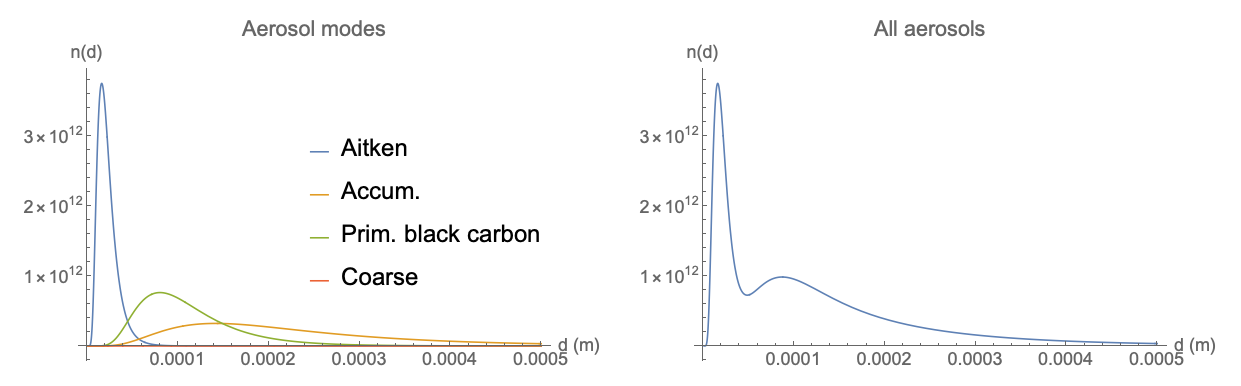
\includegraphics[width=\textwidth]{figures/pdf_examples}
\caption{Normalized size distributions $n_i$ for each mode in the Haero model
with $N_i$ set by the \texttt{num\_aer} variable.}\label{fig:mode_dists}
\end{figure}

The logarithmic form $\hat{n}_i$ is useful because of the relationship
$ n_i(D_p) = \hat{n}_i(\ln D_p)/D_p$, which allows us to write
\begin{equation} \labeleq{equ_norm_lognorm}
  n_i(D_p) \d{D_p} = \hat{n}_i(\ln D_p) \d{\ln D_p}
\end{equation}
to simplify integrands involving number distribution functions.
The benefit of this log-normal functional form choice is that the moment integrals can be defined analytically, obviating the need for potentially costly numerical quadrature \cite[eqns.~(3.7)]{Whitby1991}.
The $k$th moment is given in this case by,
\begin{equation}
  M_k^{(i)} = N_i D_{g,i}^k \exp\left(\frac{k^2}{2}\log^2\sigma_{g,i}\right).
\end{equation}

In particular,
\begin{subequations}
  \begin{align}
    M_0^{(i)} &= \int_0^\infty n_i(D_p)\,d D_p = N_i,\\
    M_1^{(i)} &= \int_0^\infty D_p n_i(D_p)\,d D_p = N_iD_{g,i}\exp({\frac{1}{2}\log^2\sigma_{g,i}}),\\
    M_2^{(i)} &= \int_0^\infty D_p^2n_i(D_p)\,d D_p = N_iD_{g,i}^2\exp(2\log^2\sigma_{g,i}),\\
    M_3^{(i)} &= \int_0^\infty D_p^3n_i(D_p)\,d D_p = N_iD_{g,i}^3\exp(\frac{9}{2}\log^2\sigma_{g,i})
  \end{align}
\end{subequations}


\begin{defn}[Particle size]
  Particle size $\overline{D_i}$ for the $i$th mode is defined by the arithmetic mean diameter associated with the 3rd moment \cite[eqn.~(1)]{Whitby1981}, 
  \begin{equation}
    \overline{D_i} = \left(M_3^{(i)}/N_i)\right)^{1/3} = D_{g,i}\exp\left(\frac{3}{2}\log^2\sigma_{g,i}\right)
  \end{equation}
\end{defn}

\begin{assume}[Particles have spherical shapes] Aerosol particles are spherical, and their size can be parameterized by their diameter $\overline{D_i}$.
The corollaries for area and volume follow, $\overline{A_i} = \pi\overline{D_i}^2$, $\overline{V_i} = \frac{\pi}{6}\overline{D_i}^3$.
\end{assume}
\pbc{I can't make a consistent $\overline{D_i}$ work with more than one $k>0$ moment. Indeed, even \cite[eqn.~(1)]{Whitby1981} notes that this choice must be associated with a specific moment. 
To see this, check: 
$$\overline{D_i}^3 \ne M_3^{(i)}/N_i. $$
The factors multiplying $\log^2\sigma_{g,i}$ do not match.
\\
Perhaps we get away with this incongruity because MAM really only used $M_{0,3}^{(i)}$ and ignores the first and second moments?
}


%\pbc{I've verified the above equations (11), which correspond to \cite[eqns.~(3.7)]{Whitby1991}, but I haven't yet figured out how they relate to $\bar A_i$, $\bar D_i$, and $\bar V_i$, unless: 
%  $$\overline{D_i} = D_{g,i}\exp(\frac{1}{2}\log^2\sigma_{g,i}),~~\overline{A}_i = \pi D_{g,i}^2\exp(2\log^2\sigma_{g,i}),~~ \overline{V_i} = \frac{\pi}{6}D_{g,i}^3\exp(\frac{9}{2}\log^2\sigma_{g,i}).$$
%  In any case, I don't know where the constant exponential factors go.
%  They remain, for example, in \cite[eqn.~(1)]{Whitby1981}.
%}

When we adopt the log-normal assumption, we express our solution for particles in
mode $i$ in terms of its zeroth, first, second, and third moments
$\mathcal{M}_k^{(i)}(\vec{x}, t)$. These are, respectively:
\begin{itemize}
  \item $\mathcal{M}_0^{(i)} = N_i$, the total number of concentration for particles
        in mode $i$
  \item $\mathcal{M}_1^{(i)} = N_i\overline{D}_i$, the number-weighted mean diameter of
        particles in mode $i$
  \item $\mathcal{M}_2^{(i)} = \frac{1}{\pi}N_i\overline{A}_i$, a number-weighted
        surface area of particles in mode $i$
  \item $\mathcal{M}_3^{(i)} = \frac{6}{\pi}N_i\overline{V}_i$, a number-weighted
        volume of particles in mode $i$
\end{itemize}

In this language, the aerosol evolution equation for the $k$th moment of the
$i$th mode is

\begin{equation}\labeleq{modal_evolution}
  \partialt{\mathcal{M}_k^{(i)}} = F_k^{(i)}(N_i, \overline{D}_i, \overline{A}_i, \overline{V}_i, T, p, \mathsf{...})
\end{equation}

where the air temperature $T$ and the air pressure $p$ enter the moment
equations, via right hand side terms in \refeq{moments}. These are the
{\bf modal equations}.

\begin{assume}[Parmeterization assumption]
   The time evolution of a moment $\mathcal{M}_k^{(i)}$ can be
    expressed in terms of the quantities $N_i$, $\overline{D}_i$,
    $\overline{A}_i$, $\overline{V}_i$, the air temperature $T$, the pressure $p$, and a few
    selected additional quantities.
\end{assume}

\begin{assume}[2-moment scheme]
  Aerosol dynamics can be represented well by two moments, $M_0^{(i)}$ and $M_3^{(i)}$.
  We therefore need to find equations that describe the time evolution of $M_0^{(i)}$ and $M_3^{(i)}$ in terms of known E3SM variables.
  \begin{itemize}
    \item The number of moles of aerosol per kg of air is $N_i/N_A$, where $N_A$ is the Avogadro Constant.
    \item The mass mixing ratio of aerosol (kg aer.\,/ kg air) is therefore $\displaystyle q^{(i)} = \frac{N_i M_w}{N_A} = \frac{\mathcal{M}_0^{(i)}M_w}{N_A}$, where $M_w$ is the molecular weight (kg/mol) of the aerosol particles in mode $i$.
    \item The mass density of aerosol particles in mode $i$ is therefore, $\rho_{aer}^{(i)} =\rho_{air} \;q^{(i)}$.
    \item The total mass of aerosol particles is then $\displaystyle M_{aer}^{(i)}=\rho_{aer}^{(i)} \overline{V_i} = \frac{\pi}{6}\frac{\rho_{aer}^{(i)}\mathcal{M}_3^{(i)}}{\mathcal{M}_0^{(i)}}$.
  \end{itemize}
\end{assume}

%Solving the closure problem is then reduced to finding expressions for
%$\overline{D}_i$, $\overline{A}_i$, and $\overline{V}_i$ that relate the
%different moments of $n_i$:
%
%\begin{align}
%  \overline{D}_i &= \overline{D}_i(\mathcal{M}_{k_1}^{(i)}/N_i, \mathcal{M}_{k_2}^{(i)}/N_i) \labeleq{D_i}\\
%  \overline{A}_i &= \overline{A}_i(\mathcal{M}_{k_1}^{(i)}/N_i, \mathcal{M}_{k_2}^{(i)}/N_i) \labeleq{A_i}\\
%  \overline{V}_i &= \overline{V}_i(\mathcal{M}_{k_1}^{(i)}/N_i, \mathcal{M}_{k_2}^{(i)}/N_i) \labeleq{V_i}
%\end{align}
%
%Here, we formulate the above expressions by the selecting pairs of moments that
%contribute to the evolution of each quantity for mode $i$.
%
%\begin{assume}[Moment pairs]
% The averaged quantities $\overline{D}_i$, $\overline{A}_i$,
%    and $\overline{V}_i$ can each be expressed as a function of a pair of
%    specific number-normalized moments for the $i$th mode.
%\end{assume}

\subsubsection*{Mode definitions in MAM4}

The choices of size range and width for the modes in MAM are based on
measurements of tropospheric aerosols (see~\cite{Easter2004} and references therein).
Table~\ref{tab:mode_size_parameters} shows the relevant parameters for MAM4,
the 4-mode legacy MAM model.

%------------------- table: mode parameters ---------------
\begin{table}[htbp]
\centering
%\caption{
%Geometric mean dry diameter ($D\dsub{gn,d,i}$, unit:
%$\rm \mu m$) and geometric standard deviation ($\sigma\dsub{g,i}$)
%of the number size distribution of each log-normal mode.
%}
%\begin{tabular}{ccccc}
%  \toprule
%  Mode        &  Lower bound of $D\dsub{gn,d,i}$  &  $D\dsub{gn,d,i}$   &
%  Upper bound of $D\dsub{gn,d,i}$  &  $\sigma\dsub{g,i}$ \\
%  \midrule
%  Aitken 	            &  0.0087  &   0.026   &   0.052  &  1.6 \\
%  Accumulation     &  0.0535  &   0.11      &   0.44    &  1.8 \\
%  Coarse               &  1.0        &   2.0       &   4.0      &  1.8 \\
%  Primary carbon  &  0.01      &   0.05      &   0.1      &  1.6 \\
%  \bottomrule
%\end{tabular}
\caption{Parameters of log-normal modes in MAM4.}
\label{tab:mode_size_parameters}
\begin{tabular}{cccccc}
  \toprule
  Mode           &  Lower bound of $D\dsub{gn,d,i}$
                 &  Upper bound of $D\dsub{gn,d,i}$  &  $\sigma\dsub{g,i}$ 
                 & $N_i(0)$\\
  \midrule
  Aitken 	 &  0.0087  &   0.052  &  1.6     & 7.9031E7\\
  Accumulation   &  0.0535  &   0.44   &  1.8 & 7.9697E7\\
  Coarse         &  1.0     &   4.0    &  1.8 & 8.0361E7\\
  Primary carbon &  0.01    &   0.1    &  1.6 & 8.1022E7\\
  \bottomrule
\end{tabular}
\end{table}
%-------------

Thus, in MAM, all modes have the same mathematical form, but the parameters
are different for each mode.

\subsection*{Multi-Species Modes}

We have derived the modal equations assuming that each mode contains a
population of undifferentiated aerosol particles. 
We assume that each particle is composed of several, potentially different, chemical species, which corresponds to the following assumption.
%If we wish to track individual
%particle species within a mode, we may do so by expressing the population of a
%mode as the sum of its constituent species in the modal assumption, adding
%a species index $s$ to the number distribution function $n$:
%
%\begin{equation}\labeleq{modal_multi_species}
%  n(\vec{x}, t; D_p) = \sum_{i=1}^M \sum_{s=1}^S n_{i,s}(\vec{x}, t; D_p)
%\end{equation}
%
%with $S$ as the number of species. Then we can carry out the subsequent analysis
%as before, breaking up the moments into species-specific parts
%$\mathcal{M}_k^{(i,s)}$ and expressing the total $k$th moment as the sum of these
%parts:
%
%\begin{equation}
%  \mathcal{M}_k^{(i)} = \sum_{s=1}^S \mathcal{M}_k^{(i,s)}
%\end{equation}
%
%Then the multi-species modal evolution equations are
%
%\begin{equation}\labeleq{modal_multi_species_evolution}
%  \partialt\mathcal{M}_k^{(i,s)} = F_k^{(i,s)}(N_{i,s}, \overline{D}_{i,s}, \overline{A}_{i,s}, \overline{V}_{i,s}, T, p, \mathsf{...})
%\end{equation}
%
%with species-specific equivalents of the quantities in \refeq{modal_evolution}.

\begin{assume}[Internally mixed]
  All aerosol species within a mode are assumed to be carried uniformly by all particles represented by the mode's log-normal distribution function, i.e., within each mode, particles are internally mixed.
\end{assume}

\begin{assume}[Additive particle volume]
  Quantitatively, the internal mixing assumption implies that the volume of each individual particle is the sum of the volumes of its various constituents; in this case, the species within the mode.  
\end{assume}

These assumption has several implications:
\begin{enumerate}
  \item All species within mode $i$ share the same particle size distribution; as a corollary, they also share the same number concentration,
  \begin{equation}
    N_{i,q} = M_0^{(i)} = N_i,
  \end{equation}
  for all species $q$ in mode $i$.
\end{enumerate}


\chapter{The Haero Library}
\labelchapter{library}

In this chapter, we describe the Haero software library itself, and its usage
within an atmospheric model.

\section{Overview}
\labelsection{lib:overview}

Haero is designed to provide a modal aerosol capability to an atmospheric model
written in C++ and/or Fortran. It makes no attempt to describe or evolve any
atmospheric phenomena outside of aerosols. Instead, Haero evolves the state of
aerosols within a modal aerosol model as part of a broader atmospheric
{\bf host model}---a mathematically consistent description of the atmosphere.

To use Haero in your own host model, you write code to interact to construct
a modal aerosol system and invoke aerosol processes on that system. Haero gives
you all the flexibility and control you need to define how the aerosol processes
couple with and interoperate with the other processes in the host model. In this
sense, Haero is a set of building blocks you can use to construct the most
appropriate modal aerosol representation for your host model.

\subsection{Aerosol Systems}
\labelsubsection{lib:systems}

Haero's representation of aerosols relies on a set of elementary data structures
that define the assumptions underlying a specific modal aerosol system. These
elements are:

\begin{itemize}
  \item An {\bf Aerosol Model}: the definition of a specific modal aerosol
        system to be simulated
  \item {\bf Modes}: statistical representations of aerosol particle populations
        organized by particle size
  \item {\bf Species}: aerosol and gas molecules of interest. Each aerosol
        species belongs to a single aerosol mode and is tracked by mass and
        number.
\end{itemize}

These entities define the aerosol system of interest in Haero, and provide
any related {\bf metadata} needed to make decisions about how an aerosol
processes does its work.

\subsection{Aerosol State Data}
\labelsubsection{lib:state}

Haero deals with two distinct types of state variables:

\begin{itemize}
  \item {\bf Prognostic variables}: variables that are evolved in time according
        to a system of differential equations
  \item {\bf Diagnostic variables}: variables that are algebraically related to
        other variables, whether those variables are prognostic or diagnostic
\end{itemize}

Prognostic variables are quantities that possess an initial state and are
evolved forward in time by their {\bf tendencies} (time derivatives). It is
not possible to construct the value of a prognostic variable at time $t$ without
an initial condition at some time $t_0$ and a tendency defined over the period
$\left[t_0, t\right]$.

The concept of a ``diagnostic'' variable is more general than its name suggests.
The word "diagnostic" suggests that the variable is used only as an indicator
by a human attempting to ``diagnose'' some atmospheric condition. In fact, a
diagnostic variable can be any variable whose state can be constructed at any
instant in time, using only the relevant prognostic variables.

Haero's aerosol state data lives in multi-dimensional arrays within ``smart
containers'' called \verb Prognostics  and \verb Diagnostics , whose names
indicate the types of variables they store. These arrays are stored in
\verb View  data structures provided by the Kokkos C++ library. Aerosol state
data is allocated in C++, but available for use in Fortran for implementing
aerosol processes or for using Haero from within a Fortran host model.

\subsection{Aerosol Processes}
\labelsubsection{lib:processes}

The aerosol ``life cycle'' consists of a set of complicated physical processes
involving many participants, with a wide range of length and time scales. These
different scales demand a degree of flexibility in how we evaluate changes to
the state of an aerosol system. For example, we expect to be able to resolve
processes whose time scale is similar to or larger than the time scale for
convection in the atmosphere, whereas processes with faster time scales must be
treated in some special way that accommodates a relaxation or equilibration
process.

Haero provides data structures for constructing two distinct types of aerosol
processes:

\begin{itemize}
  \item A {\bf prognostic process} accepts a set of prognostic and diagnostic
        variables as input, and computes as output one or more tendencies for a
        corresponding set of prognostic variables. It does not make any changes
        to any of its inputs.
  \item A {\bf diagnostic process} accepts a set of prognostic variables as
        input, and updates one or more diagnostic variables in place so that
        these variables are consistent with the prognostic variables.
\end{itemize}

A process consists of a set of parameterizations that encode simplifying
assumptions about a specific stage of the aerosol life cycle into an algorithm
that computes the relevant quantities of interest. The processes provided by
Haero, and their various parameterizations, are described in \refchapter{processes}.

These processes are the true assets of the Haero library. They can be
implemented in C++, in Fortran, or in both. This allows aerosol researchers to
make their latest parameterizations available in the Haero library, while
providing software engineers with a ``future-proof'' environment for optimizing
these and other parameterizations for DOE's Leadership Class Facilities.

That's an orbit-level view of the Haero library. Now let's take a closer look at
each of these aspects.

\section{Aerosol Systems in Haero}
\labelsection{lib:systems}

To model a specific aerosol system in Haero, we must answer some questions:

\begin{itemize}
  \item What modes are required to accurately characterize the distribution of
        interesting particle sizes?
  \item What species are present in the system, and in what modes are they
        allowed to appear?
  \item How many atmospheric columns are needed to model the system?
  \item How many vertical levels are needed to resolve the profile of aerosols
        in the system?
  \item Which physical processes are relevant to a simulation of interest?
        Should any processes be excluded, to answer a specific question about
        how the processes interact with each other, or because they are not
        signficant for the system?
\end{itemize}

Each of these decisions greatly affects the nature of the model---systems with
different answers to these questions will have very different behavior. When we
define a Haero simulation, we encode the answers to these decisions in an
{\bf aerosol model} variable.

What do we mean by an ``aerosol model'', exactly? One can think about it in a
few different ways.

\begin{itemize}
  \item An aerosol model specifies the physics (or the approximations to the
        physics, if you like) represented by an aerosol simulation.
  \item An aerosol model stores a set of ``global variables'' that govern the
        behavior for the simulation of a single aerosol system.
  \item Every aerosol system is described by exactly one aerosol model.
  \item The aerosol model encodes the assumptions made about an aerosol system's
        representation. It does not define the state of that system at any given
        time. In this sense, all of its information is ``timeless''.
\end{itemize}

\subsection{The Model Type}
\labelsubsection{lib:model}

In Haero, an aerosol model is defined by the \verb Model  type, defined within
the \verb haero  namespace. Interfaces to this type are provided in both C++ and
Fortran.

Below is an abbreviated look at the \verb Model  C++ class. The source code for
this class can be found in the \verb haero/model.hpp  and
\verb haero/model.cpp files within the repository. Reading through this class,
you'll see references to various other data structures. We describe these data
structures in subsequent sections.

\begin{verbatim}
class Model final {
  public:

  // Constructor -- creates a new model given all relevant data.
  Model(const Parameterizations& parameterizations,
        const std::vector<Mode>& aerosol_modes,
        const std::vector<Species>& aerosol_species,
        const std::map<std::string, std::vector<std::string> >& mode_species,
        const std::vector<Species>& gas_species,
        int num_columns,
        int num_levels);

  // Creates a set of prognostic variables for use with this model.
  Prognostics* create_prognostics() const;

  // Creates a set of diagnostic variables for use with this model.
  Diagnostics* create_diagnostics() const;

  // Runs the (prognostic) aerosol process of the given type, computing any
  // relevant tendencies.
  void run_process(ProcessType type,
                   Real t, Real dt,
                   const Prognostics& prognostics,
                   const Diagnostics& diagnostics,
                   Tendencies& tendencies);

  // Runs the (diagnostic) aerosol process of the given type, updating all
  // relevant diagnostic variables in place.
  void update_diagnostics(ProcessType type, Real t,
                          const Prognostics& prognostics,
                          Diagnostics& diagnostics);

  // Returns the parameterizations associated with this aerosol model.
  const Parametrizations& parametrizations() const;

  // Returns the list of modes for the context.
  const std::vector<Mode>& modes() const;

  // Returns the list of aerosol species for the context.
  const std::vector<Species>& aero_species() const;

  // Returns the list of gas species for the context.
  const std::vector<Species>& gas_species() const;

  // Returns the number of vertical atmospheric columns in a simulation
  // associated with this context.
  int num_columns() const;

  // Returns the number of vertical levels (cells) in each atmospheric column.
  int num_levels() const;
};
\end{verbatim}

In C++, you can create as many \verb Model  variables as you like, though
there's usually no reason to do so, unless you're running an ensemble of
simulations whose underlying assumptions differ beyond their initial states.

Haero's Fortran interface provides a \verb model_t  derived type with a subset
of the information available to the C++ \verb Model  type. While the Fortran
interface doesn't have ``feature parity'' with its C++ counterpart, we argue
that it provides ample information for implementing aerosol processes in
Fortran.

\begin{verbatim}
type :: model_t
  ! The aerosol modes in the model, in indexed order.
  type(mode_t), dimension(:), allocatable :: modes
  ! The number of modes in the model. Equal to size(modes).
  integer :: num_modes
  ! The number of actual species that exist within each mode.
  integer, dimension(:), allocatable :: num_mode_species
  ! The aerosol species within each mode. Indexed as (mode, species).
  type(species_t), dimension(:,:), allocatable :: aero_species
  ! The gas species in the model.
  type(species_t), dimension(:), allocatable :: gas_species
  ! The number of columns in the model.
  integer :: num_columns
  ! The number of vertical levels in each column.
  integer :: num_levels
end type
\end{verbatim}

In Fortran, a single global \verb model_t  variable, \verb model , is provided
within the \verb haero  module. This variable is automatically populated with
data by Haero before any work is done, so there's no need to create it or
modify it yourself. {\em Do not attempt to change any data within
this global variable}.

Because the model definition is provided as a global variable, only one instance
of an aerosol model is available to Fortran implementations of aerosol processes.

\subsection{The Mode Type}
\labelsubsection{lib:modes}

We've seen how the dynamics of aerosols can be represented mathematically
by evolution equations for moments of modal distribution functions. Modes
simplify the description of aerosol particles in terms of their size: instead of
representing a population of particles with a distribution function
$n(V_p, \vec{x}, t)$ that varies continuously with the size of the particle, we
introduced $M$ discrete modes and declared that these modes partition the
population of aerosol particles in the sense of the modal assumption as given
by \refeq{modal_n}.

The essential information in a mode is the range of particle sizes it
encompasses, $[D_{\min}, D_{\max}]$, and its geometric standard deviation,
$\sigma_g$. In Haero's C and C++ interfaces,
we represent an aerosol mode with the \verb|Mode| struct:

\begin{verbatim}
struct Mode {
  std::string name;  // a unique identifier for the mode
  Real min_diameter; // the mode's minimum particle diameter
  Real max_diameter; // the mode's maximum particle diameter
  Real mean_std_dev; // the geometric mean standard deviation for the mode
};
\end{verbatim}

Haero's Fortran interface offers a \verb mode_t  data structure, equivalent to
the C++ \verb Mode  class. This data structure is defined in the \verb haero  Fortran
module:

\begin{verbatim}
type :: mode_t
  ! Mode name
  character(len=:), allocatable :: name
  ! Minimum particle diameter
  real(wp) :: min_diameter
  ! Maximum particle diameter
  real(wp) :: max_diameter
  ! Geometric mean standard deviation
  real(wp) :: mean_std_dev
end type
\end{verbatim}

In principle, a Haero calculation can support any number of modes, but care
must be taken to ensure that the modal assumptions remain valid, and that
the parametrizations selected can accommodate the given modes.

\subsection{The Species Type}
\labelsubsection{lib:species}

Each aerosol mode consists of one or more particle species. Additionally,
gas particles also come in different species. Both aerosol particles and
gas particles have physical properties that are described by the
\verb Species  data type.

A particle species is a specifically-identified molecular assembly with
a number of relevant physical properties. The fundamental description of a
species includes

\begin{itemize}
  \item a symbolic name (e.g. \verb SO4 , for sulfate)
  \item a descriptive name (e.g. \verb "sulfate" )
  \item information about the chemical properties of the species
\end{itemize}

In C++, we represent this information in the following way:

\begin{verbatim}
struct Species {
  std::string name;          // full species name
  std::string symbol;        // abbreviated symbolic name
  Real molecular weight;     // molecular weight [g/mol]
  Real crystalization_point; // crystalization point [?]
  Real deliquescence_point;  // deliquenscence point [?]
};
\end{verbatim}

In Fortran, a species is defined by the following derived type:
\begin{verbatim}
type :: species_t
  ! Species name
  character(len=:), allocatable :: name
  ! Species symbol (abbreviation)
  character(len=:), allocatable :: symbol
  ! Molecular weight [g/mol]
  real(wp) :: molecular_wt
  ! Crystalization point [?]
  real(wp) :: crystal_pt
  ! Deliquenscence point [?]
  real(wp) :: deliques_pt
end type
\end{verbatim}

\section{State Variables in Haero}
\labelsection{lib:state}

Once a model variable has been created that defines an aerosol system, you can
create state variables for that system. The state of a system is defined by the
following prognostic variables:

\begin{itemize}
  \item {\bf modal number densities}: the total number of particles per cubic
        meter in each mode
  \item {\bf aerosol modal mix fractions}: the fraction of a mode occupied
        by each aerosol species present within that mode
  \item {\bf gas mole fractions}: the number of moles of each gas species per
        mole of air
\end{itemize}

In addition, the model possesses a set of diagnostic variables that depend on
its selected aerosol processes (which are discussed in a later section).

How does one create a set of state variables given a model variable? Recall that
the \verb Model  C++ class provides the following two functions, which you can
call directly yourself, given a pointer to a C++ variable called \verb model :

\begin{itemize}
  \item \verb model->create_prognostics()  : returns a pointer to a C++
    \verb Prognostics  container
  \item \verb model->create_diagnostics()  : returns a pointer to a C++
    \verb Diagnostics  container
\end{itemize}

These functions don't take any parameters---they just use the information within
the model variable.

By the way, you don't always have to call these functions yourself. State
variables are automatically created if you're using the Haero driver or
implementing a parameterization in C++ or Fortran. However, if you're using
Haero within your own host model, or if you're writing a unit test for your
parameterization, you must call these functions to obtain containers for your
aerosol model's state data.

The \verb Prognostics  and \verb Diagnostics  containers store prognostic and
diagnostic state data, respectively, in multidimensional arrays allocated in C++
but made available to both C++ and Fortran. The data for each array is stored
within a Kokkos View.

\subsection*{Kokkos Views}
\labelsubsection{lib:views}

The C++ programming language has lots of features, but remarkably it includes no
mechanism for allocating multidimensional arrays at runtime. The Kokkos C++
library fills this gap by providing a data structure called a \verb View . A
\verb View  is essentially an interface that allows a C++ programmer to treat a
chunk of memory like a multidimensional array.

A \verb View  has a rank and a set of dimensions, just like an allocatable
Fortran array. You access a \verb View  in the same way that you'd access a
Fortran array, except that C++ uses row-major indexing instead of Fortran's
column-major indexing. So for a rank-3 view \verb f  that you access in C++
as \verb f(i,j,k) , you would access the corresponding array in Fortran as
\verb f(k,j,i) .

{\em TODO: try to make some sense of packs}

Because Haero is concerned with arrays having very specific dimensions, we
define some named types that correspond to views/arrays that span specific
spaces:

\begin{table}[htbp]
\centering
\caption{Named C++ View Types}
\label{tab:viewtypes}
\begin{tabular}{|l|l|l|l|l|}
  \toprule
  View Name & Rank & Description & C++ & Fortran \\
  \midrule
  \verb ColumnView  & 2 & Maps a column $i$ and a vertical level $k$ to a pack & \verb v(i,k)  & \verb v(k,i) \\
  \verb ColumnSpeciesView  & 3 & Maps a column $i$, a vertical level $k$, and a species $s$ to a pack & \verb v(i,k,s)  & \verb v(s,k,i) \\
  \verb ModalColumnView & 3 & Maps a mode index $m$, a column $i$, and a vertical level $k$ to a pack & \verb v(i,k,s)  & \verb v(s,k,i) \\
  \bottomrule
\end{tabular}
\end{table}

Both the \verb Prognostics  and \verb Diagnostics  containers described below
make use of these named types.

\subsection{Prognostics Type}
\labelsubsection{lib:prognostics}

The \verb Prognostics  C++ class provides access to the prognostic variables
that define aerosols in a modal description. Here's the C++ class interface
(abbreviated for brevity---see the full interface in \verb haero/prognostics.hpp ):

\begin{verbatim}
class Prognostics final {
  public:
  // Returns the number of aerosol modes in the system.
  int num_aerosol_modes() const;

  // Returns the number of aerosol species in the mode with the given index.
  int num_aerosol_species(int mode_index) const;

  // Returns the number of gas species in the system.
  int num_gas_species() const;

  // Returns the number of independent atmospheric columns in the system.
  int num_columns() const;

  // Returns the number of vertical levels per column in the system.
  int num_levels() const;

  // Returns the view storing interstitial aerosol species mixing fraction data
  // for the mode with the given index.
  const ColumnSpeciesView& interstitial_aerosols(int mode_index) const;

  // Returns the view storing cloud-borne aerosol species mixing fraction data
  // for the mode with the given index.
  const ColumnSpeciesView& cloudborne_aerosols(int mode_index) const;

  // Returns the view storing the mole fractions of gas species in the state.
  const ColumnSpeciesView& gas_mole_fractions() const;

  // Returns the view storing the modal number densities.
  const ModalColumnView& modal_num_densities() const;

  // Scales the given set of tendencies and adds it into this state, summing
  // the values of the prognostic variables in place.
  void scale_and_add(Real scale_factor, const Tendencies& tendencies);
};
\end{verbatim}

Typically, you never modify a \verb Prognostics  variable directly. Instead, you
compute a set of tendencies (in a \verb Tendencies  variable, which is very
similar to a \verb Prognostics  variable) and accumulate them into your
\verb Prognostics  variable by calling \verb scale_and_add .

The Fortran version of the \verb Prognostics  type is similar, and offers
access to Fortran multidimensional arrays instead of C++ views. For cleaner
syntax, this type uses bound procedures to return pointers to its arrays.

\begin{verbatim}
  type :: prognostics_t
  contains
    ! Access to interstitial aerosol mix fractions array
    procedure :: interstitial_aerosols => p_int_aero_mix_frac
    ! Access to cloudborne aerosol mix fractions array
    procedure :: cloudborne_aerosols => p_cld_aero_mix_frac
    ! Access to gas mole fractions array
    procedure :: gas_mole_fractions => p_gas_mole_frac
    ! Access to modal number densities array
    procedure :: modal_num_densities => p_modal_num_densities
  end type

  ! Provides access to the interstitial aerosol mixing fractions array
  ! for the given mode in the given prognostics object p.
  function p_int_aero_mix_frac(p, mode) result(retval)
    class(prognostics_t), intent(in)  :: p
    integer(c_int), value, intent(in) :: mode
    real(c_real), pointer, dimension(:,:,:) :: retval
  end function

  ! Provides access to the cloud-borne aerosol mixing fractions array
  ! for the given mode in the given prognostics object p.
  function p_cld_aero_mix_frac(p, mode) result(retval)
    class(prognostics_t), intent(in)  :: p
    integer(c_int), value, intent(in) :: mode
    real(c_real), pointer, dimension(:,:,:) :: retval
  end function

  ! Provides access to the gas mole fractions array for the given
  ! prognostics object p.
  function p_gas_mole_frac(p) result(retval)
    use iso_c_binding, only: c_ptr, c_int
    class(prognostics_t), intent(in) :: p
    real(c_real), pointer, dimension(:,:,:) :: retval
  end function

  ! Provides access to the modal number fractions array for the given
  ! prognostics object p.
  function p_modal_num_densities(p) result(retval)
    use iso_c_binding, only: c_ptr, c_int
    class(prognostics_t), intent(in) :: p
    real(c_real), pointer, dimension(:,:,:) :: retval
  end function

\end{verbatim}

\subsection{Diagnostics Type}
\labelsubsection{lib:diagnostics}

The \verb Diagnostics  C++ class stores a dynamically-determined set of
diagnostic variables that correspond to the specific parameterizations available
to the aerosol model that created it.

\begin{verbatim}
class Diagnostics final {
  public:
  // Returns the number of aerosol modes in the system.
  int num_aerosol_modes() const;

  // Returns the number of aerosol species in the mode with the given index.
  int num_aerosol_species(int mode_index) const;

  // Returns the number of gas species in the system.
  int num_gas_species() const;

  // Returns the number of independent atmospheric columns in the system.
  int num_columns() const;

  // Returns the number of vertical levels per column in the system.
  int num_levels() const;

  // Returns true if the given (non-modal) variable exists within this object,
  // false otherwise.
  bool has_var(const std::string& name) const;

  // Returns the view storing the diagnostic variable with the given name.
  // If the variable does not yet exist, this throws an exception.
  ColumnView& var(const std::string& name);

  // Returns true if the given modal aerosol variable exists within this object,
  // false otherwise.
  bool has_aerosol_var(const std::string& name) const;

  // Returns the view storing the modal aerosol diagnostic variable with the
  // given name and mode index. If the variable does not yet exist, this throws
  // an exception.
  ColumnSpeciesView& aerosol_var(const std::string& name, int mode_index);

  // Returns true if a variable defined for each gas species exists within
  // this object with the given name, false otherwise.
  bool has_gas_var(const std::string& name) const;

  // Returns the view storing a diagnostic variable, defined for each gas
  // species, with the given name. If the variable does not yet exist, this
  // throws an exception.
  ColumnSpeciesView& gas_var(const std::string& name);

  // Returns true if the given modal variable exists within this object,
  // false otherwise.
  bool has_modal_var(const std::string& name) const;

  // Returns the view storing the mode-specific diagnostic variable with the
  // given name. If the variable does not yet exist, this throws an exception.
  // @param [in] name The name of the diagnostic variable.
  ModalColumnView& modal_var(const std::string& name);
};
\end{verbatim}

The Fortran version of \verb Diagnostics , like its \verb Prognostics  counterpart,
uses bound procedures to provide access to its array data:

\begin{verbatim}
  type :: diagnostics_t
  contains
    procedure :: has_var => d_has_var
    procedure :: var => d_var
    procedure :: has_aerosol_var => d_has_aerosol_var
    procedure :: aerosol_var => d_aerosol_var
    procedure :: has_gas_var => d_has_gas_var
    procedure :: gas_var => d_gas_var
    procedure :: has_modal_var => d_has_modal_var
    procedure :: modal_var => d_modal_var
  end type

  ! Returns true if the given diagnostics object d contains a (non-modal)
  ! variable with the given name, false otherwise.
  function d_has_var(d, name) result(retval)
    use iso_c_binding, only: c_ptr, c_bool
    class(diagnostics_t), intent(in) :: d
    character(len=*), intent(in) :: name
    logical(c_bool) :: retval
  end function

  ! Provides access to the given (non-modal) variable in the given
  ! diagnostics object d.
  function d_var(d, name) result(retval)
    class(diagnostics_t), intent(in)  :: d
    character(len=*), intent(in) :: name
    real(wp), dimension(:,:), pointer :: retval
  end function

  ! Returns true if the given diagnostics object d contains a modal aerosol
  ! variable with the given name, false otherwise.
  function d_has_aerosol_var(d, name, mode) result(retval)
    use iso_c_binding, only: c_ptr, c_char, c_bool, c_int
    class(diagnostics_t), intent(in) :: d
    character(len=*), intent(in) :: name
    integer(c_int), intent(in) :: mode
    logical(c_bool) :: retval
  end function

  ! Provides access to the given (non-modal) variable in the given
  ! diagnostics object d.
  function d_aerosol_var(d, name, mode) result(retval)
    class(diagnostics_t), intent(in)  :: d
    character(len=*), intent(in) :: name
    integer(c_int), intent(in) :: mode
    real(wp), dimension(:,:,:), pointer :: retval
  end function

  ! Returns true if the given diagnostics object d contains a (non-modal)
  ! variable with the given name, false otherwise.
  function d_has_gas_var(d, name) result(retval)
    use iso_c_binding, only: c_ptr, c_bool
    class(diagnostics_t), intent(in) :: d
    character(len=*), intent(in) :: name
    logical(c_bool) :: retval
  end function

  ! Provides access to the given (non-modal) variable in the given
  ! diagnostics object d.
  function d_gas_var(d, name) result(retval)
    class(diagnostics_t), intent(in)  :: d
    character(len=*), intent(in) :: name
    real(wp), dimension(:,:,:), pointer :: retval
  end function

  ! Returns true if the given diagnostics object d contains a modal
  ! variable with the given name, false otherwise.
  function d_has_modal_var(d, name) result(retval)
    use iso_c_binding, only: c_ptr, c_bool
    class(diagnostics_t), intent(in) :: d
    character(len=*), intent(in) :: name
    logical(c_bool) :: retval
  end function

  ! Provides access to the given modal variable in the given
  ! diagnostics object d.
  function d_modal_var(d, name) result(retval)
    class(diagnostics_t), intent(in)  :: d
    character(len=*), intent(in) :: name
    real(wp), dimension(:,:,:), pointer :: retval
  end function

\end{verbatim}

At this point, you might wonder how a \verb Diagnostics  variable knows which
variables it needs. In fact, the \verb Diagnostics  class provides functions for
creating variables that it needs. The C++ \verb Model  variable used to create
a \verb Diagnostics  variable knows this information, and automatically calls
these functions for you.

For examples of how these \verb Prognostics  and \verb Diagnostics  types are
used in practice, take a look at one of the existing aerosol process
implementations.

\section{Aerosol Processes in Haero}
\labelsection{lib:processes}

The aerosol life cycle consists of several important and distinct physical
processes. As we mentioned in \refsubsection{lib:processes}, there are
{\bf prognostic processes}, which compute tendencies for prognostic variables,
and there are {\bf diagnostic processes}, which update diagnostic variables
in place.

Haero offers data structures that make it very easy to implement these two types
of processes. Because the structure of a given process doesn't depend on the
details of its implementation, we can define abstract interfaces for these
processes. These abstract interfaces simplify the development of a process---
instead of designing a new process from the ground up every time you want to
add new functionality to Haero, you can simply implement a small number of
functions (or subroutines) that define the behavior of a process, and let the
Haero library handle the details of how these processes are created and used.

For detailed descriptions of the specific processes provided by Haero, take a
look at \refchapter{processes}. You can find examples of source code for
Haero's processes in the \verb haero/processes  subdirectory.

\subsection{The Prognostic Process Interface}
\labelsubsection{lib:prognostic_process}

A prognostic process has three behaviors which must be defined by any
implementation. Each of these behaviors is implemented in a C++ function or
a Fortran subroutine.

\begin{enumerate}
  \item {\bf initialization}: the process must be able to allocate any resources
        it needs to do its work. These resources include temporary work arrays,
        look-up tables, and quantities that need to be precomputed. State data
        is not managed by processes, so it's not included in process
        initialization. If nothing needs to be done for initialization, its
        function or subroutine body can be empty.
  \item {\bf running}: the process must know how to ``run''. In other words, it
        must define a procedure for computing tendencies for a relevant set of
        prognostic variables given their current values, and the current values
        of any diagnostic variables. The function or subroutine that implements
        this behavior does not apply these tendencies to any prognostic
        variables---it simply computes the tendencies and returns.
  \item {\bf finalization}: at the end of a simulation program, when the aerosol
        system is destroyed, the process must free all resources it allocated
        in its initialization. If no resources are allocated, the function or
        subroutine body implementing finalization can be empty.
\end{enumerate}

Haero provides an object-oriented approach for implementing a process in terms
of this simple interface. In an object-oriented approach, an abstract interface
is encoded in a ``base class''---a data type that declares the necessary
functions and subroutines. Then any implementation of this interface is defined
in a data type ``derived'' from that base class.

Haero uses the object-oriented features of C++ for process development. All
prognostic process implementations are derived from a C++ base class called
\verb PrognosticProcess . This is true regardless of whether you implement the
process using C++ or Fortran.

The \verb PrognosticProcess  provides the following interface (see
\verb haero/process.hpp  for more details):

\begin{verbatim}
class PrognosticProcess {
  public:

  // Constructor, called by all PrognosticProcess subclasses.
  PrognosticProcess(ProcessType type, const std::string& name):
    type_(type), name_(name) {}

  // Destructor.
  virtual ~PrognosticProcess() {}

  // Override this method if your aerosol process needs to be initialized
  // with information about the model. The default implementation does nothing.
  virtual void init(const Model& model) {}

  // Override this method to implement the aerosol process using the specific
  // parameterization for the subclass.
  virtual void run(const Model& model,
                   Real t, Real dt,
                   const Prognostics& prognostics,
                   const Diagnostics& diagnostics,
                   Tendencies& tendencies) const = 0;
};
\end{verbatim}

In addition to the ``constructor'' function used to create an instance of a
\verb PrognosticProcess  variables, this interface declares three functions
(\verb init , \verb run , and the destructor function \verb \~PrognosticProcess )
that correspond to the three behaviors described above.

The constructor accepts a process type that indicates what stage of the aerosol
life cycle it represents. A \verb ProcessType  data structure is an
``enumerated type'' that enumerates the various stages:

\begin{verbatim}
// This enumerated type lists all relevant physical aerosol processes.
enum ProcessType {
  ActivationProcess,
  CloudBorneWetRemovalProcess,
  CoagulationProcess,
  CondensationProcess,
  DryDepositionProcess,
  EmissionsProcess,
  InterstitialWetRemovalProcess,
  NucleationProcess,
  ResuspensionProcess,
  WaterUptakeProcess
};
\end{verbatim}

Let's explore how we might implement a prognostic aerosol process in C++ and in
Fortran. Here we describe only the steps needed to implement the process itself.
You must also testing your process to make sure it behaves the way you think it
does! The procedure for testing an aerosol process is described in
\refchapter{testing}.

\subsubsection{C++ prognostic processes}
\labelsubsubsection{lib:prognostic_cxx}

In C++, all you have to do in order to implement a prognostic process is to
define a class with a specific name, derived from the
\verb PrognosticProcess  base class. For example, the MAM4 implementation of the
nucleation process, described in \refsubsection{nuc:mam4}, is defined in a C++
class named \verb MAM4NucleationProcess . A C++ class derived from a base class
is called a {\bf subclass} of that base class, so
\verb MAM4NucleationProcess  is a subclass of \verb PrognosticProcess .

To create a C++ implemention for a prognostic process:

\begin{enumerate}
  \item Create a header file that declares your subclass of
        \verb PrognosticProcess . This header file must declare a constructor,
        a destructor, the \verb init  function, and the \verb run  function.
        This file lives in the \verb haero/processes  subdirectory within the
        repository. See \verb haero/processes/MAM4NucleationProcess.hpp  for an
        example.
  \item Create a source file containing implementations for the constructor, the
        destructor, the \verb init  functon, and the \verb run  function for
        your subclass. This lives alongside the header file you just created.
        See \verb haero/processes/MAM4NucleationProcess.cpp for an example.
        In particular, select the \verb ProcessType  value that reflects the
        proper stage of the aerosol lifecycle for your process.
  \item Add your source file to the set of source files in the
        \verb PROCESS_SOURCES  variable in \verb haero/processes/CMakeLists.txt .
  \item Write one or more tests for your new aerosol process.
        \refchapter{testing} provides extensive details about how to do this.
\end{enumerate}

\subsubsection{Fortran prognostic processes}
\labelsubsubsection{lib:prognostic_f90}

A Fortran prognostic process implementation consists of a C++ class derived
from the \verb FPrognosticProcess  base class. Here, your C++ subclass is a
very thin wrapper around three Fortran subroutines that live in their own
module. For an example of how this looks in practice, take a look at the
\verb MAM4NucleationFProcess  defined in the following files:

\begin{itemize}
  \item \verb haero/processes/MAM4NucleationFProcess.hpp : the C++ wrapper class
        declaration
  \item \verb haero/processes/MAM4NucleationFProcess.cpp : the C++ wrapper class
        implementation, which calls the subroutines in the associated
        Fortran module. This source file must declare the names of the Fortran
        subroutines in an {\verb extern "C"} block in order for them to be
        visible to the C++ compiler.
  \item \verb haero/processes/mam4_nucleation.F90 : the Fortran submodule, which
        defines the three subroutines called by the C++ wrapper class. These
        subroutines must be declared with the {\verb bind(c) } attribute, and
        must have the same name as those declared in the {\verb extern "C"}
        block in the C++ wrapper class implementation.
\end{itemize}

In other words, an aerosol process implemented in Fortran must have a C++ class
that calls a set of Fortran subroutines. The \verb FPrognosticProcess  C++ class
takes care of most of the work needed for C++ and Fortran to communicate with
each other---all you have to do is supply the Fortran subroutines in a module,
and declare these subroutines in your class implementation.

In this sense, the procedure for creating a Fortran implementation of an aerosol
process is very similar to that for a C++ implementation:

\begin{enumerate}
  \item Create a header file that declares your subclass of
        \verb FPrognosticProcess . Unlike a C++ implementation, this subclass
        only needs a constructor function---the rest of the interface is handled
        by logic in the \verb FPrognosticProcess  class. Like a C++
        implementation, this header file lives in the
        \verb haero/processes  subdirectory within the repository.
  \item Create a Fortran module in which you define three subroutines that
        implement the \verb init , \verb run , and \verb finalize  behaviors
        for your process. Make sure these subroutines are public, and declare
        them with the \verb bind(c)  attribute to make them accessible to C++.
        This module lives in \verb haero/processes  with your C++ header file.
  \item Create a source that contains an implementation for the constructor
        function you declared in the header file above. In this constructor,
        you must call the constructor for the \verb FPrognosticProcess  class.
        The arguments to this constructor include the type and name of the
        process, and the three Fortran subroutines you defined in your module.
        behaviors. These subroutines must be declared in an {\verb extern "C"}
        block within this file. The source file lives alongside the header file
        and the Fortran module you created.
  \item Add your C++ source file and Fortran module to the set of source files
        in the \verb PROCESS_SOURCES  variable in
        \verb haero/processes/CMakeLists.txt .
  \item Write one or more tests for your new aerosol process.
\end{enumerate}

\subsubsection{Making your prognostic process available to Haero}

So you've implemented your prognostic process in C++ or Fortran. How do you
make it available to the Haero library? There are a few more things you need to
do before Haero can construct a model that includes your new process type:

\begin{enumerate}
  \item Edit the \verb SelectedProcesses  struct in
        \verb haero/selected_processes.hpp  , and add a field to the enumerated
        type that corresponds to the \verb ProcessType  value you selected in
        Step 2 of your implementation procedure above.
  \item Edit the \verb select_prognostic_process  function in
        \verb haero/selected_processes.cpp  to create a new pointer to your
        process type.
  \item Update the driver YAML input parser to add an option for a user
        to select your new process.
  \item Update this document with a description of your process in the
        appropriate section of \refchapter{processes}.
\end{enumerate}

Once you've done these things and rebuilt Haero, your new process type is
available for use.

\subsection{The Diagnostic Process Interface}
\labelsubsection{lib:diagnostic_process}

Like a prognostic process, a diagnostic process has three behaviors that must be
implemented in a C++ function or a Fortran subroutine.

\begin{enumerate}
  \item {\bf initialization}: like a prognostic process, a diagnostic process
        can perform whatever work and/or resource allocation is needed during
        initialization. If nothing needs to be done for initialization, its
        function or subroutine body can be empty.
  \item {\bf updating}: the process must know how to update any relevant
        diagnostic variables. The procedure for updating these variables is
        defined by a function or subroutine that provides all prognostic
        variables for the aerosol system as input. The function or subroutine
        that implements this behavior updates the relevant diagnostic variables
        immediately and returns.
  \item {\bf finalization}: the finalization of a diagnostic process is similar
        to that for a prognostic process. If no resources are allocated by the
        process during initialization, the function or subroutine body
        implementing finalization can be empty.
\end{enumerate}

Implementing a diagnostic process is very similar to implementing a prognostic
process. The only difference is that the diagnostic process has an
\verb update  behavior with a different interface from the \verb run  behavior
in a prognostic process.

As in the case of prognostic processes, we use C++'s object-oriented approach to
implement diagnostic processes in C++ and Fortran. This time we derive a C++
class from the \verb DiagnosticProcess  base class, which has following
interface (see \verb haero/process.hpp ):

\begin{verbatim}
class DiagnosticProcess {
  public:

  // Constructor, called by all DiagnosticProcess subclasses.
  DiagnosticProcess(ProcessType type, const std::string& name):
    type_(type), name_(name) {}

  // Destructor.
  virtual ~DiagnosticProcess() {}

  // Override this method if your aerosol process needs to be initialized
  // with information about the model. The default implementation does nothing.
  virtual void init(const Model& model) {}

  // Override this method to update diagnostic variables at the given time.
  virtual void update(const Model& model, Real t,
                      const Prognostics& prognostics,
                      Diagnostics& diagnostics) const = 0;

  // This function accepts the names of diagnostic variables required by this
  // process. These variables include those variables used by the process, as
  // well as variables computed by the process. The process ensures that any
  // Diagnostics object passed to it has storage for these variables. This
  // is usually called inside the constructor of a DiagnosticProcess subclass.
  void set_diag_vars(const std::vector<std::string>& vars,
                     const std::vector<std::string>& aero_vars,
                     const std::vector<std::string>& gas_vars,
                     const std::vector<std::string>& modal_vars);
};
\end{verbatim}

Everything about this interface is the same as the \verb PrognosticProcess ,
except that

\begin{itemize}
  \item the \verb run  function here is replaced by the \verb update  function
  \item there's a \verb set_diag_vars  function that you can use to express
        which diagnostic variables are required by your process
\end{itemize}

The procedure for implementing a diagnostic process is almost exactly
the same as that for a prognostic process.

\subsubsection{Implementing a diagnostic process in C++}
\labelsubsubsection{lib:diagnostic_cxx}

To create a C++ implemention for a diagnostic process:

\begin{enumerate}
  \item Create a header file that declares your subclass of
        \verb DiagnosticProcess . This header file must declare a constructor,
        a destructor, the \verb init  function, and the \verb run  function.
        This file lives in the \verb haero/processes  subdirectory within the
        repository. See \verb haero/processes/MAM4WaterUptakeProcess.hpp  for an
        example.
  \item Create a source file containing implementations for the constructor, the
        destructor, the \verb init  functon, and the \verb run  function for
        your subclass. This lives alongside the header file you just created.
        See \verb haero/processes/MAM4WaterUptakeProcess.cpp for an example.
        In particular, select the \verb ProcessType  value that reflects the
        proper stage of the aerosol lifecycle for your process.
  \item If your diagnostic process requires the presence of specific diagnostic
        variables, call the \verb set_diag_vars  function (with the appropriate
        variable names of each type) in the class's constructor.
  \item Add your source file to the set of source files in the
        \verb PROCESS_SOURCES  variable in \verb haero/processes/CMakeLists.txt .
  \item Write one or more tests for your new aerosol process.
        \refchapter{testing} provides extensive details about how to do this.
\end{enumerate}

\subsubsection{Implementing a diagnostic process in Fortran}
\labelsubsubsection{lib:diagnostic_f90}

A Fortran diagnostic process implementation consists of a C++ class derived
from the \verb FDiagnosticProcess  base class. As in the case of prognostic
processes, your C++ subclass is a thin wrapper around three Fortran subroutines
that live in their own module. This is illustrated in the
\verb MAM4WaterUptakeFProcess  defined in the following files:

\begin{itemize}
  \item \verb haero/processes/MAM4WaterUptakeFProcess.hpp : the C++ wrapper class
        declaration
  \item \verb haero/processes/MAM4WaterUptakeFProcess.cpp : the C++ wrapper class
        implementation, which calls the subroutines in the associated
        Fortran module. This source file must declare the names of the Fortran
        subroutines in an {\verb extern "C"} block in order for them to be
        visible to the C++ compiler.
  \item \verb haero/processes/mam4_water_uptake.F90 : the Fortran submodule, which
        defines the three subroutines called by the C++ wrapper class. These
        subroutines must be declared with the {\verb bind(c) } attribute, and
        must have the same name as those declared in the {\verb extern "C"}
        block in the C++ wrapper class implementation.
\end{itemize}

Again, the \verb FDiagnosticProcess  C++ class takes care of most of the work
needed for the C++/Fortran bridge. You simply supply the Fortran subroutines in
a module, and declare these subroutines in your class implementation.

So, to create a Fortran implementation for a diagnostic process:

\begin{enumerate}
  \item Create a header file that declares your subclass of
        \verb FDiagnosticProcess . Once again, this subclass needs only a
        constructor function. This header file lives in the
        \verb haero/processes  subdirectory within the repository.
  \item Create a Fortran module in which you define three subroutines that
        implement the \verb init , \verb update , and \verb finalize  behaviors
        for your process. Make sure these subroutines are public, and declare
        them with the \verb bind(c)  attribute to make them accessible to C++.
        This module lives in \verb haero/processes  with your C++ header file.
  \item Create a source that contains an implementation for the constructor
        function you declared in the header file above. In this constructor,
        you must call the constructor for the \verb FDiagnosticProcess  class.
        The arguments to this constructor include the type and name of the
        process, and the three Fortran subroutines you defined in your module.
        behaviors. These subroutines must be declared in an {\verb extern "C"}
        block within this file. The source file lives alongside the header file
        and the Fortran module you created.
  \item Make sure you call \verb set_diag_vars  in your C++ class's constructor
        function to list the diagnostic variables needed by your process.
  \item Add your C++ source file and Fortran module to the set of source files
        in the \verb PROCESS_SOURCES  variable in
        \verb haero/processes/CMakeLists.txt .
  \item Write one or more tests for your new aerosol process.
\end{enumerate}

\subsubsection{Making your diagnostic process available to Haero}

To make Haero aware of your new diagnostic process, you follow similar steps
to those for prognostic processes:

\begin{enumerate}
  \item Edit the \verb SelectedProcesses  struct in
        \verb haero/selected_processes.hpp  , and add a field to the enumerated
        type that corresponds to the \verb ProcessType  value you selected in
        Step 2 of your implementation procedure above.
  \item Edit the \verb select_diagnostic_process  function in
        \verb haero/selected_processes.cpp  to create a new pointer to your
        process type.
  \item Update the driver YAML input parser to add an option for a user
        to select your new process.
  \item Update this document with a description of your process in the
        appropriate section of \refchapter{processes}.
\end{enumerate}

It's helpful to look at examples of existing prognostic and diagnostic
processes before you get started on your own. In addition, it often helps to
think about how you might test a process to clarify and test your assumptions.
In the next chapter, we discuss Haero's approach to testing aerosol processes.

\chapter{Testing Aerosol Processes}
\labelchapter{testing}


\chapter{Available Aerosol Processes}
\labelchapter{processes}

Haero offers implementations for each of the important stages in the aerosol
life cycle. Here we describe the physics of each stage, the approximations
made by the associated parametrizations, and the implementations of the
underlying prognostic and diagnostic processes.

In each of the processes, we assume the state of an aerosol system is specified
by the following prognostic variables:

\begin{itemize}
  \item $ n_m(x_i, y_i, z_k, t)$ [\# /m$^3$]: the {\em number density} of mode $m$,
        defined within the cell in column $i$ at vertical level $k$
  \item $ q_{m,s}(x_i, y_i, z_k, t)$ [kg aerosol species $s$/kg air]: the
        {\em mass mix fraction} of aerosol species $s$ within mode $m$, defined
        within the cell in column $i$ at vertical level $k$
  \item $ q_g(x_i, y_i, z_k, t)$ [kmol gas species $g$/mkol air]: the {\em mole
        fraction} of gas species $g$, defined within the cell in column $i$ at
        vertical level $k$
\end{itemize}

Further, each process is independent of all other processes. In other words,
state variables are taken directly from the prognostics and diagostics passed
to the process, and no assumptions are made about how these state variables
were computed.

\begin{assume}[Independent aerosol processes]
  Every aerosol process is independent of other aerosol processes. Specifically:
  a process takes a set of state variables and diagnostics, and {\em using only
  these variables}, performs one of the following procedures, based on its
  process type:
  \begin{enumerate}
    \item If the process is {\em prognostic}, it computes a set of tendencies
          for the prognostic state variables at simulation time $t$.
    \item If the process is {\em diagnostic}, it updates any relevant diagnostic
          variables in place at simulation time $t$.
  \end{enumerate}
\end{assume}

This process independence is a dramatic departure from prior implementations of
aerosol physics in MAM. Any sequential coupling of processes must be performed
by a host model.

With this assumption, it's possible to recover the legacy MAM algorithms by
constructing a coupling procedure that follows the relevant assumptions. But
it's also possible to construct more sophisticated coupling processes that take
advantage of advances in numerical analysis.

\section{Nucleation}
\labelsection{nucleation}

Aerosol nucleation refers to the formation of new aerosol particles from gas
molecules. Nucleation is an important source of aerosol particles in the
atmosphere, and can have a significant effect on other aerosol-related
processes. As a conversion mechanism, it reduces the population of gas-phase
species and increases aerosol mass and number concentrations.

Aerosol nucleation can also affect the formation of clouds and fog. The newly
formed particles that result from nucleation are generally hydrophilic and not
efficiently scavenged because of their small sizes. These particles can
grow larger and act as nuclei for cloud condensation.

Haero currently offers one process implementation for nucleation: the legacy
MAM4 model, written in Fortran.

\subsection{Nucleation Physics}
\labelsubsection{nuc:physics}

In the atmosphere, gas molecules exist either independently or in small
polymolecular clusters~\cite{seinfeld-2006-acp}. In general, the concentration
of independent gas molecules is much higher than that of clusters. Therefore,
the radius of a cluster is changed mainly due to the collision between an
independent gas molecule and a cluster. If the radius of a cluster is larger
than $r^*$, the radius of the so-called ``critical cluster'' or nucleus, this
cluster tends to grow rapidly and nucleation happens; otherwise, this cluster
tends to shrink and nucleation does not occur.

Nucleation can occur {\em homogeneously} (in the absence of pre-existing
particles) or {\em heterogeneously} (with pre-existing particles present).
In either case, nucleation can involve a single species or more than one species.
Based on these circumstances, we can classify any nucleation process:

\begin{itemize}
  \item {\bf Type 1} nucleation is homogeneous and involves a single species.
  \item {\bf Type 2} nucleation is homogeneous and involves two or more species,
        e.g. water vapor ($\rwater$) and sulfuric acid gas ($\rsag$).
  \item {\bf Type 3} nucleation is heterogeneous and involves a single species.
        A good example is the formation of water droplets in the presence of
        pre-existing particles.
  \item {\bf Type 4} nucleation is heterogeneous and involves two or more
        species.
\end{itemize}

In all four cases, the nucleation process alters the vapor mixing ratios and
aerosol mass and number mixing ratios. Their rates of change are

\begin{align}
  \ddt{q_{m,s}} &= \ddt{q_{n,s}} \cdot \frac{m_{d,s}}{\mu_{s}} \,, \labeleq{nuc:aer}\\
  \ddt{q_g}     &= -\ddt{q_{m,s}} \,, \labeleq{nuc:gas}
\end{align}

where
\begin{itemize}
  \item $q_{m,s}$ [kmol aerosol species $s$/ kmol dry air] is the aerosol mass
        mixing ratio of species $s$
  \item $q_{n,s}$ [\# aerosol species $s$/ kmol dry air] is the aerosol number
        mixing ratio for species $s$
  \item $q_g$ [kmol gas species $g$/ kmol dry air] is the mole fraction for gas
        species $g$
  \item $m_{d,s}$ [kg] is the dry mass of a nucleus belonging to aerosol species
        $s$
  \item $\mu_{s}$ [kg/kmol] is the molecular weight of aerosol species $s$
\end{itemize}

% key assumptions
\subsection{MAM4 Nucleation Process}
\labelsubsection{nuc:mam4}

Although we have mentioned four types of aerosol nucleation, the MAM4 nucleation
process treats only type 2. MAM4 makes several assumptions on top of the modal
aerosol assumption to arrive at its governing equations for nucleation:

\begin{assume}[MAM4 Nucleation: Aitken mode]
  There is no nucleation mode---instead, the Aitken mode is used to capture the
  smallest nucleated aerosol particles.
\end{assume}

Previous research~\cite{kerminen-2002-jas} suggests that the typical size
range of newly formed nuclei are around 1 nm in diameter.

\begin{assume}[MAM4 Nucleation: new nucleus size]
  Newly formed nuclei have a 1 nm diameter.
\end{assume}

Particles of this size are too small to be represented directly by MAM4's Aitken
mode. To reconcile this difficulty with its modal approximation, the MAM4
process breaks nucleation into two distinct stages.

\begin{assume}[MAM4 Nucleation: separate creation and growth stages]
  The nucleation process consists of two stages:
  \begin{enumerate}
    \item Fresh nuclei are formed from the vapors of gas species.
    \item These nuclei grow to a predefined size that falls within the range
      of the Aitken mode. This predefined size is described in
      \refparagraph{nuc:growth_nuclei}.
  \end{enumerate}
  Therefore, nucleation affects only the aerosol number and mass mixing ratios
  in the Aitken mode.
\end{assume}

\begin{assume}[MAM4 Nucleation: gas/aerosol density]
  In the MAM4 nucleation process, the mass densities of aerosol sulfuric acid
  and sulfate are assumed to be the same: $\rm 1770~kg~m^{-3}$
\end{assume}

\begin{assume}[MAM4 Nucleation: averaged $\rsag$ number concentration]
  To calculate the number concentration of $\rsag$ [\# / cc air], we use
  $c\dsub{n,\sag}$, the average mass mixing ratio of $\rsag$ over the
  condensation process. We use $c\dsub{n, \sag}$ instead of the mass mixing
  ratio of $\rsag$ given at the beginning of the nucleation process.

  $$c\dsub{n,\sag} = 10^{-3} \cdot N_A \cdot \bar{q_{\sag}} c\dsub{air}$$

  where $N_A$ is Avogadro's constant and $c\dsub{air}$ [kmol air / m$^3$ air] is
  the air molar concentration.
\end{assume}

\begin{assume}[MAM4 Nucleation: homogeneous only]
  MAM4 treats only the homogeneous nucleation of $\rsag \mhyphen \rwater$
  (type 2).
\end{assume}

With these assumptions, the governing equations of MAM4's nucleation process
are

\begin{align}
  \frac{dq\dsub{n,i}}{dt} &= \frac{10^6 J\dsub{nuc}}{c\dsub{air}} \,, \text{ i = 2 for Aitken mode} \,, \labeleq{nuc:jnuc} \\
  \frac{d\amass{\asf}}{dt} &= \frac{dq\dsub{n,i}}{dt} \cdot \frac{m\dsub{d,\asf}}{\mu_{\asf}} \,, \text{ i = 2} \,, \labeleq{nuc:amass} \\
  \frac{d\vmass{\sag}}{dt} &= -\frac{d\amass{\asf}}{dt} \,, \text{ i = 2} \,, \labeleq{nuc:vmass}
\end{align}

where $J\dsub{nuc}$ [\# / (cc $\cdot$ s)] is the nucleation rate describing the
net number of clusters that grow past $r^*$ per unit time per cm$^{3}$ of
air. $J\dsub{nuc}$ depends on the available amount of gas species, temperature
and relative humidity.

% parameterization
\subsubsection{MAM4 nucleation parameterizations} \labelsubsubsection{nuc:paranuc}

In order to solve the above governing equations, one first computes $J\dsub{nuc}$,
which appears in \refeq{nuc:jnuc}. In principle, $J\dsub{nuc}$ can be calculated
thermodynamically by classical nucleation theory, which is described in
Chapter 11 of~\cite{seinfeld-2006-acp}. However, this classical treatment
carries a heavy computational cost and is not used in the MAM4 model. Instead,
we devise parameterizations to obtain $J\dsub{nuc}$.

Here we focus on the parameterizations of binary nucleation of
$\rsag \mhyphen \rwater$ used in MAM4.

The following notation simplifies our presentation:
\begin{itemize}
  \item RH: clear-sky relative humidity.
  %\item $c\dsub{n,\sag}$ [\# / cc air]: number concentration of $\rsag$.
  \item $n\dsub{\sag}$ [\#]: number of $\rsag$ molecules in a critical cluster.
  \item $n\dsub{tot}$ [\#]: number of molecules in a critical cluster.
  \item $J^*$ [\# / (cc $\cdot$ s)]: the {\em intermediate nucleation rate},
        which is modified by a sequence of parameterizations
        (\refparagraph{nuc:binary} -~\refparagraph{nuc:growth_nuclei}) to
        obtain $J\dsub{nuc}$.
  \item $C\dsub{sum,\sag}$ [s$^{-1}$]: the sum of mass transfer coefficients of
        $\rsag$ over the $I$ modes during the condensation process. This is a
        constant for the nucleation process.
\end{itemize}

With this assumption, the following nucleation parameterizations are evaluated
in order. First, RH is bounded within [0.01, 0.99] since the nucleation process
in MAM4 is only considered for clear-sky conditions. In clouds, $\rsag$
rapidly transfers into cloud droplets, and nucleation is unlikely to occur.

% binary nucleation parameterization by vk2002
\paragraph{Binary nucleation of $\rsag \mhyphen \rwater$}
\labelparagraph{nuc:binary}

MAM4 uses the binary parameterization developed by
Vehkam\"aki et al.~\citep{vehkamaki-2002-jgr}. This parameterization fits $J^*$
to a polynomial function of $T$, $RH$ and $c\dsub{n,\sag}$. This representation
is valid under the following conditions:

\begin{itemize}
  \item $T \in [230.15, 305.15]$;
  \item $RH \in [0.0001, 1.0]$;
  \item $c\dsub{n,\sag} \in [10^4, 10^{11}]$;
  \item $J^* \in [10^{-7}, 10^{10}]$;
\end{itemize}

Only the \textbf{first three} constraints are actually applied in the MAM4
process. $T$ and $RH$ are bounded within the given range. If
$c\dsub{n,\sag} \le 10^4$ or $\vmass{\sag,avg} \le 4 \cdot 10^{-16}$
(two roughly equivalent conditions), nucleation is assumed to not occur,
$J\dsub{nuc}$ is set to $0$ in \refeq{nuc:jnuc}, and the calculation
terminates.

If the above conditions are satisfied, this parameterization computes the
following quantities in order:

\begin{enumerate}
  \item The mole fraction of $\rsag$ in a critical cluster (i.e., $x^*$) is
        given by:
    \begin{align}
      x^* &= 0.740997 - 0.00266379 T - 0.00349998 \ln c\dsub{\sag}
             + 0.0000504022 T \ln c\dsub{\sag} \nonumber \\
          &+ 0.00201048 \ln RH - 0.000183289 T \ln RH
             + 0.00157407 (\ln RH)^2 \nonumber \\
          &- 0.0000179059 T (\ln RH)^2 + 0.000184403 (\ln RH)^3 \nonumber \\
          &- 1.50345 \cdot 10^{-6} T (\ln RH)^3 \,.
    \end{align}
  \item The intermediate nucleation rate (i.e., $J^*$) is calculated from
        $x^*$:
        \begin{align}
          J^* &= \exp \Big[ a(T,x^*) + b(T,x^*) \ln RH +
                 c(T,x^*) (\ln RH)^2 + d(T,x^*) (\ln RH)^3 \nonumber \\
              &+ e(T,x^*) \ln c\dsub{\sag} + f(T,x^*) (\ln RH) \ln c\dsub{\sag}
                 + g(T,x^*) (\ln RH)^2 \ln c\dsub{\sag} \nonumber \\
              &+ h(T,x^*) (\ln c\dsub{\sag})^2 + i(T,x^*) (\ln RH)
                (\ln c\dsub{\sag})^2 + j(T,x^*) (\ln c\dsub{\sag})^3 \Big] \,, \labeleq{vk2002_nucrate}
        \end{align}
        where the coefficients $a(T,x^*) \dots j(T,x^*)$ are given in
        \refappendixsubsection{nuc:coeff_nucrate}.
  \item $n\dsub{tot}$, the total number of molecules in a critical cluster,
        is calculated from $x^*$:
        \begin{align}
          n\dsub{tot} &= \exp \Big[ A(T,x^*) + B(T,x^*) \ln RH
                         + C(T,x^*) (\ln RH)^2 + D(T,x^*) (\ln RH)^3 \nonumber \\
                      &+ E(T,x^*) \ln c\dsub{\sag} + F(T,x^*) \ln RH \ln c\dsub{\sag}
                         + G(T,x^*) (\ln RH)^2 \ln c\dsub{\sag} \nonumber \\
                      &+ H(T,x^*) (\ln c\dsub{\sag})^2
                       + I(T,x^*) \ln RH (\ln c\dsub{\sag})^2
                       + J(T,x^*) (\ln c\dsub{\sag})^3 \Big] \,, \labeleq{vk2002_ntot}
        \end{align}
        where the coefficients $A(T,x^*) \dots J(T,x^*)$ are given in
        \refappendixsubsection{nuc:coeff_ntot}.
  \item $n\dsub{\sag}$, the total number of $\rsag$ molecules in a critical
        cluster, is calculated from $x^*$ and $n\dsub{tot}$:
        \begin{equation}
          n\dsub{\sag} = n\dsub{tot} x^* \,.
        \end{equation}
  \item $r^*$ [nm], the radius of a critical cluster, is calculated from
        $x^*$ and $n\dsub{tot}$:
        \begin{equation}
          r^* = \exp \left[ -1.6524245 + 0.42316402 x^* +
                0.3346648 \ln n\dsub{tot} \right] \,.
        \end{equation}
\end{enumerate}

% binary nucleation parameterization by wang2009
\paragraph{Nucleation within the planetary boundary layer} \labelparagraph{nuc:pbl}

If nucleation occurs within the planetary boundary layer (PBL) or below a
a height of 100 meters, $J^*$ is compared with $J\dsub{PBL}$, an additional
parameterization that uses an empirical first-order estimation
~\cite{sihto-2006-acp,wang-2009-acp}. Here we make an additional assumption:

\begin{assume}[MAM4 Nucleation: new nucleus composition]
  New aerosol nuclei consist entirely of $\rsag$.
\end{assume}

The empirical estimation is
\begin{equation}
  J\dsub{PBL} = 10^{-6}~c\dsub{\sag} \,.
\end{equation}

If $J\dsub{PBL} > J^*$, the the following adjustments are made:
\begin{align}
  J^* &= J\dsub{PBL} \,, \\
  r^* &= 0.5~nm \,, \\
  n\dsub{\sag} &= \frac{6.023 \times 10^{23} \pi (1~nm)^3
                  \rho\dsub{\sag}}{6 \mu_{\sag}} \,, \\
  n\dsub{tot} &= n\dsub{\sag} \,.
\end{align}

Otherwise, $J^*$, $n\dsub{tot}$ and $n\dsub{\sag}$ remain the same values
calculated by the first parameterization in \refparagraph{nuc:binary}.

% parameterization of nuclei growth
\paragraph{Nuclei growth} \labelparagraph{nuc:growth_nuclei}

If $J^* < 10^{-6}$ based on the previous calculations, nucleation does not
occur.

\begin{assume}[MAM4 Nucleation: nucleation rate cutoff]
  If $J^*$, the intermediate nucleation rate, is less than $10^{-6}$ molecules
  per cc per second, based on binary nucleation and PBL effects, then no
  nucleation occurs.
\end{assume}

Otherwise, the nucleation calculation proceeds, and the following quantities are
computed:

\begin{align}
  RH &\in [0.1, 0.95] \,, \\
  f\dsub{v} &= 1 - \frac{0.56}{\ln RH} \,, \\
  V\dsub{d,nuc} &= \frac{n\dsub{\sag} \mu_{\asf}}
                   {6.023 \cdot 10^{26} \rho\dsub{\sag}} \,, \\
  D\dsub{d,nuc} &= \left( \frac{6 V\dsub{d,nuc}}{\pi} \right)^{\frac{1}{3}} \,,
\end{align}

where

\begin{itemize}
  \item $f\dsub{v}$ is the ratio of wet volume over dry volume of a particle,
        using a simple K\"ohler approximation for $\rm NH\dsub{4}HSO\dsub{4}$
  \item $V\dsub{d,nuc}$ [$\rm m^3$] $D\dsub{d,nuc}$ [m] are the dry volume and
        diameter of a nucleus, estimated from the binary nucleation and PBL
        parameterizations
\end{itemize}

The simplified approximation for $f\dsub{v}$ follows the K\"ohler theory used by
the MAM4 aerosol water uptake, but neglects surface curvature effects. The
composition is assumed to be pure ammonium bisulfate with hygroscopicity = 0.56.

To decide whether the nuclei have grown large enough to fit within the Aitken
mode's acceptible range of sizes, we use this mode's predefined min, max, and
mean particle diameters [m] to calculate two quantities:
\begin{align}
  D\dsub{p,lo} &= \exp \left[ 0.67 \ln (8.7 \cdot 10^{-9}) +
                            0.33 \ln (26 \cdot 10^{-9}) \right] \,, \\   %% about 12.5 nm
  D\dsub{p,hi} &= 52 \cdot 10^{-9} \,.
\end{align}
\textcolor{red}{Jian: Dick said $D\dsub{p,lo}$=8.7 nm might make more sense.}

If $D\dsub{d,nuc} > D\dsub{p,lo}$, $J\dsub{nuc}$ is set to $J^*$. Otherwise,
the nuclei are too small for the Aitken mode. We use the following
parameterization to consider the growth of nuclei to a larger size
\cite{kerminen-2002-jas}. This parameterization makes the following assumptions:

\begin{assume}[MAM4 Nucleation: no self-coagulation]
  The only significant ``sink'' mechanism for new aerosol nuclei is their
  coagulation with pre-existing particles. In other words, the MAM4 model
  ignores the self-coagulation of fresh aerosol nuclei.
\end{assume}

\begin{assume}[MAM4 Nucleation: growth by constant condensation]
  The only important source for the growth of nuclei is the condensation
  of vapors, and this condensation rate is assumed to be constant.
\end{assume}

\begin{assume}[MAM4 Nucleation: static growth process]
  The population of pre-existing particles and the concentration of
  condensible vapors remain unchanged during the growth process for new
  nuclei.
\end{assume}

\begin{assume}[MAM4 Nucleation: non-volatile vapors]
  The condensable vapors responsible for nuclei growth are non-volatile.
\end{assume}

Using this parameterization, we adjust $J^*$ based on

\begin{itemize}
  \item the increase of the size of nuclei due to condensation of $\rsag$
  \item the decrease of the number concentration of nuclei due to
        coagulation with pre-existing particles
\end{itemize}

The following quantities are calculated in the following order for the
adjustment of $J^*$:

\begin{align}
  v\dsub{\sag} &= 14.7 \sqrt{T} \,, \\
  \rho\dsub{nuc} &= \frac{\rho\dsub{\sag}}{f\dsub{v}} \,, \\
  GR &= \frac{3.0 \cdot 10^{-9} v\dsub{\sag} \mu_{\sag} c\dsub{n,\sag}}
        {\rho\dsub{nuc}} \,, \\
  D\dsub{nuc,ini} &= \max (2r^*, 1) \,, \\
  D\dsub{nuc,fin} &= 10^9 D\dsub{p,lo} f\dsub{v}^{\frac{1}{3}} \,, \\
  \gamma &= 0.23 D\dsub{nuc,int}^{0.2}
                 (\frac{D\dsub{nuc,fin}}{3})^{0.075}
                 (\frac{\rho\dsub{nuc}}{1000})^{-0.33}
                 (\frac{T}{293})^{-0.75} \,, \labeleq{nuc:gamma} \\
  \mathbb{D}\dsub{g,\sag} &= \frac{6.7037 \cdot 10^{-9} T^{0.75}}
                             {c\dsub{air}} \,, \\
  CS^\prime &= \frac{C\dsub{sum,\sag}}
               {4 \pi \mathbb{D}\dsub{g,\sag} \alpha\dsub{\sag}} \,, \label{eq:cs_prime} \\
  \eta &= \frac{\gamma CS^\prime}{GR} \,, \\
  J\dsub{nuc} &= J^* \exp \left( \frac{\eta}{D\dsub{nuc,fin}} -
                     \frac{\eta}{D\dsub{nuc,ini}} \right) \,,
\end{align}

where
\begin{itemize}
  \item $v\dsub{\sag}$ [m/s] is the approximated mean molecular speed of $\rsag$
  \item $\rho\dsub{nuc}$ [kg/m$^3$] is the mass density of nuclei after
        accounting for aerosol water uptake by sulfate
  \item $GR$ [m/s] is the nuclei growth rate, assumed to be constant
  \item $D\dsub{nuc,ini}$ [nm] and $D\dsub{nuc,fin}$ [nm] are the wet diameters
        of nuclei before and after growth
  \item $\mathbb{D}\dsub{g,\sag}$ [$\rm m^2/s$] is the approximate gas
        diffusivity of $\rsag$
  \item $CS^\prime$ is the ``condensation sink'', constant based on the
        assumption that the population of pre-existing particles does not
        change
\end{itemize}

The formula for $CS^\prime$ used in MAM4 comes from the condensation equation of
$\rsag$ gas and differs from that in~\cite{kerminen-2002-jas}. According to Dick
Easter, this difference is minor and produces no significant changes in
nucleation results.
% and the detailed derivation can be found in the Appendix~\ref{cs_prime}.
%Note that compared with the Eq. (22) in~\cite{kerminen-2002-jas},
%Dick also dropped a term in \refeq{nuc:gamma}, which was
%thought to be close to 1.

\subsubsection{MAM4 nucleation: numerical considerations}

After $J\dsub{nuc}(t\dsub{0})$ is calculated using the parameterizations in
\refsubsubsection{nuc:paranuc}, $\Delta \aitmass{\asf}$---the increase of
$\aitmass{\asf}$ due to nucleation---can be calculated:
%
\begin{align}
  \Delta \aitmass{\asf} &= \frac{10^6 J\dsub{nuc}(t\dsub{0}) \Delta t\dsub{nuc} m\dsub{d,\asf}}
                            {c\dsub{air}\mu_{\asf}} \,, \\
  m\dsub{d,\asf} &= \begin{cases}
    \rho\dsub{\sag} \frac{\pi}{6}V\dsub{p,hi}^3 \,, \, \text{if $D\dsub{d,nuc} \ge D\dsub{p,hi}$} \,, \\
    \rho\dsub{\sag} \frac{\pi}{6}V\dsub{d,nuc}^3 \,, \, \text{if $D\dsub{p,hi} > D\dsub{d,nuc} > D\dsub{p,lo}$} \,, \\
    \rho\dsub{\sag} \frac{\pi}{6}V\dsub{p,lo}^3 \,, \, \text{otherwise} \,,
  \end{cases}
\end{align}

where $\Delta t\dsub{nuc}$ = $t\dsub{1}$ - $t\dsub{0}$ = $\Delta t\dsub{phys}$.

%(See ``MAM\_Basics'' documentation for the value of $\Delta t\dsub{phys}$).
Since $\Delta \aitmass{\asf}$ cannot exceed the available amount of
$\vmass{\sag}(t\dsub{0})$, we apply a limiting factor $f^*$, computed
as the following fraction:

\begin{equation}
  f^* = \begin{cases}
        \frac{\vmass{\sag}(t\dsub{0})}{\Delta \aitmass{\asf}}, \, \text{if $\Delta \aitmass{\asf} > \vmass{\sag}(t\dsub{0})$} \,, \\
        1, \text{otherwise.} \\
  \end{cases}
\end{equation}

If $J\dsub{nuc} f^* < 10^{-18}$, $J\dsub{nuc}$ is set to $0$ and no nucleation
occurs. Otherwise, we make the following adjustments:

\begin{align}
  \Delta \aitmass{\asf} &= \min ( 0.9999\vmass{\sag}(t\dsub0), f^* \Delta \aitmass{\asf} ) \,, \\
  \Delta \vmass{\sag} &= - \Delta \aitmass{\asf} \,, \\
  \Delta q\dsub{n,2} &= \frac{\Delta \aitmass{\asf} \mu_{\asf}}{m\dsub{d,\asf}} \,.
\end{align}

If $\frac{\Delta q\dsub{n,2}}{\Delta t\dsub{nuc}} < 100$, no nucleation occurs.
Otherwise we continue with the following adjustments:

\begin{itemize}
  \item If $\frac{\Delta \aitmass{\asf} \mu_{\asf}}{\Delta q\dsub{n,2}} <
        \frac{\pi}{6} \rho\dsub{\asf} D\dsub{p,lo}^3$, the nuclei size is
        increased at the expense of the number concentration:
        $$\Delta q\dsub{n,2} = \frac{\Delta \aitmass{\asf} \mu_{\asf}}{\frac{\pi}{6} \rho\dsub{\asf} D\dsub{p,lo}^3}$$
  \item If $\frac{\Delta \aitmass{\asf} \mu_{\asf}}{\Delta q\dsub{n,2}} >
        \frac{\pi}{6} \rho\dsub{\asf} D\dsub{p,hi}^3$, the nuclei size is
        decreased, and mass is reduced accordingly:
        $$\Delta \aitmass{\asf} = \frac{\frac{\pi}{6} \rho\dsub{\asf} D\dsub{p,hi}^3 \Delta q\dsub{n,2}}{\mu_{\asf}}$$
\end{itemize}

\jjc{This can't be the whole story---neither the number concentration nor the
mass is altered above.}

Dick commented that 1) the first ``if'' condition revealed the fact that
there was not enough $\rsag$ gas for all the nuclei to grow to the size
$D\dsub{p,lo}$. Thus Dick arbitrarily reduced the number of nuclei to
increase the size of nuclei; 2) the second ``if'' condition will never
happen, so it is just a ``sanity check''.

After the adjustment above, we solve the governing equations
\refeq{nuc:jnuc}-\refeq{nuc:vmass} numerically:

\begin{align}
  q\dsub{n,2} (t\dsub{1}) &= q\dsub{n,2} (t\dsub{0}) + \Delta q\dsub{n,2} \,, \\
  \aitmass{\asf} (t\dsub{1}) &= \aitmass{\asf} (t\dsub{0}) + \Delta \aitmass{\asf} \,, \\
%\Delta q\dsub{\sag} &= \min \left( \Delta \aitmass{\asf}, \vmass{\sag} (t\dsub{0}) \right) \,, \\
  \Delta q\dsub{\sag} &= -\Delta \aitmass{\asf} \,, \\
  \vmass{\sag} (t\dsub{1}) &= \vmass{\sag} (t\dsub{0}) + \Delta q\dsub{\sag} \,.
\end{align}

\subsubsection{Additional MAM4 nucleation diagnostics} \label{output}

The MAM4 nucleation process provides the following diagnostic variables:

\begin{enumerate}
  \item $J^*$: the nucleation rate after the first and second (if applicable)
        parameterizations
  \item $q\dsub{n,2}$: the number mixing ratio of $\rasf$ in the Aitken mode at
        $t = t\dsub1$
  \item $\vmass{\sag} (t\dsub1)$: the mass mixing ratio of $\rsag$ at
        $t = t\dsub1$
  \item $\aitmass{\asf} (t\dsub1)$: the mass mixing ratio of $\rasf$ in the
        Aitken mode at $t = t\dsub1$.
\end{enumerate}

\jjc{Here's an example of a prognostic process that computes diagnostic
variables ``along the way.'' Should we discuss whether to make these diagnostics
available to other processes?}

\subsubsection{MAM4 nucleation verification tests} \labelsubsubsection{nuc:nuctests}

The parameterizations we've described above allow us to make some general
observations about output from the MAM4 process, given valid input:

\begin{itemize}
  \item All aerosol mix fraction tendencies are zero except those for the Aitken
        mode, which are zero or positive.
  \item All modal number density tendencies are zero except those for the Aitken
        mode, which are zero or positive.
  \item All gas-phase species tendencies are non-positive. Any positive
        aerosol tendencies in the Aitken mode are associated with negative
        tendencies in gas-phase species.
  \item All newly-formed aerosol nuclei are $\rsag$ and are 1 nm in diameter.
\end{itemize}

\jjc{Can we say anything about mass conservation between gases and aerosols?}

These conditions hold for any valid input. We can say more about output for
input with given characteristics:

%\begin{itemize}
%\end{itemize}



\chapter{The Haero Driver}
\labelchapter{driver}

The standalone driver program, \texttt{haero\_driver}, provides a simple way to
explore the capabilities of Haero. It's a simple single-column model with a
bundled one-dimensional dynamics package. With it, you can

\begin{itemize}
  \item run single-column aerosol simulations
  \item perform statistical analysis on ensembles consisting of several columns
  \item conduct time-step convergence studies to build confidence in Haero's
        mathematical algorithms and their implementations
  \item select specific aerosol processes and parametrizations to examine
        in isolation, to debug or verify a given algorithm
  \item study how the aerosol processes interact with one-dimensional dynamics
        and other simplified physical process representations
\end{itemize}

In this chapter we describe the driver and its capabilities. The input format
for the driver is based on YAML and is described in \refappendix{driver_input}.

\section{Column Dynamics}

We use a one-dimensional (vertical) atmosphere and tests of increasing complexity.

Let $z=z(a,t)$ denote the trajectory of the particle labeled $a$ that arrives at physical position $z$ at time $t$.
The label $a$ is the Lagrangian, or material, coordinate. 
Particle trajectories are defined by
\begin{equation}\label{eq:traj}
\deriv{z}{t}(a,t) = w(z(a,t),t),
\end{equation}
where $w(z,t)$ is the vertical velocity.  
In the following sections, it will be convenient to formulate \eqref{eq:traj} in terms of the geopotential $\phi(a,t) = gz(a,t)$, 
\begin{equation}\label{eq:geo_traj}
  \deriv{\phi}{t}(a,t) = gw\left(\frac{\phi(a,t)}{g},t\right).
\end{equation}


Adiabatic column dynamics are described by the 1D Euler equations for a moist atmosphere,
\begin{subequations}\label{eq:1d}
  \begin{align}
    \totd{w} &= -g\left(\frac{1}{\rho}\partd{p}{\phi} + 1\right), \label{eq:momentum}\\
    \totd{\rho} &= - g\rho \partd{w}{\phi}, \label{eq:continuity}\\
    \totd{\theta_v} &= 0, \label{eq:thermo},\\
    \totd{q_v} &= 0, \label{eq:qv}
  \end{align}
\end{subequations}
where $\rho$ is density, $p$ is pressure, $\theta_v$ is the virtual potential temperature, and $q_v$ is the water vapor mass mixing ratio.
As in \cite{Taylor2020}, we treat virtual potential temperature $\theta_v$ as a material invariant.
The momentum, continuity, thermodynamic equation, and transport equation (respectfully) combine with \eqref{eq:geo_traj} and the equation of state,
\begin{equation}\label{eq:eos}
  \frac{p}{\Pi} = \rho R \theta_v,
\end{equation}
to define the complete system.
Above, $\Pi = (p/p_{ref})^{\kappa}$ is the nondimensional Exner pressure, with constant $\kappa = R/c_p$, where $R$ is the dry air gas constant and $c_p$ is the specific heat of dry air at constant pressure.
We have 6 prognostic variables: $\phi, w, \rho, \theta_v, q_v, p$, and 6 equations in \eqref{eq:geo_traj}, \eqref{eq:1d}, \eqref{eq:eos}.
The boundary conditions are $w(0,t) = w(z_{top},t) = 0$.

The advantage of the Lagrangian frame of reference imposed by \eqref{eq:geo_traj} is that the material derivative becomes an ordinary time derivative, $D/Dt = d/dt$. 
Hence, for the remainder of this note we simply use $d/dt$ in our notation.

We begin with an ansatz that the velocity has a simple form,
\begin{equation}\label{eq:z_vel}
  w(z,t) = w_0\sin\frac{\pi z}{z_{top}}\sin \frac{2\pi t}{t_p},
\end{equation}
where we have introduced parameters for the maximum velocity, $w_0$, the top of the model column, $z_{top}$, and the period of oscillation $t_p$.  
This velocity satisfies the boundary conditions and the initial condition, $w(z,0) = 0$.
We assume that this velocity is valid for all time throughout the whole column, from $z=0$ to $z=z_{top}$.
In terms of the geopotential, \eqref{eq:z_vel} becomes,
\begin{equation}\label{eq:phi_vel}
  w(\phi,t) = w_0 \sin \frac{\pi \phi}{g z_{top}}\sin\frac{2\pi t}{t_p}.
\end{equation}
Since velocity is prescribed, it does not need to be prognosed. 
This eliminates \eqref{eq:momentum} from our system of equations \eqref{eq:1d}.
Our goal is to derive the other variables associated with 1D motion in a non-hydrostatic column so that we have consistent dynamics and thermodynamics.

Substituting \eqref{eq:phi_vel} in \eqref{eq:geo_traj} we discover a separable ODE,
\begin{align}
  \deriv{\phi}{t} &= gw_0\sin\frac{\pi \phi}{g z_{top}}\sin\frac{2\pi t}{t_p},\\
  \Rightarrow \int \csc\frac{\pi \phi}{g z_{top}}\,d\phi &= g w_0\int\sin\frac{2\pi t}{t_p}\,dt,
\end{align}
whose solution is
\begin{equation}\label{eq:phi_sol}
\phi(t) = \frac{2gz_{top}}{\pi}\arctan\left[\tan\frac{\pi \phi_0}{2g z_{top}}\exp\left(\frac{w_0t_p}{z_{top}} \sin^2 \frac{\pi t}{t_p}\right)\right].
  \end{equation}

\begin{figure}[H]
  \centering
  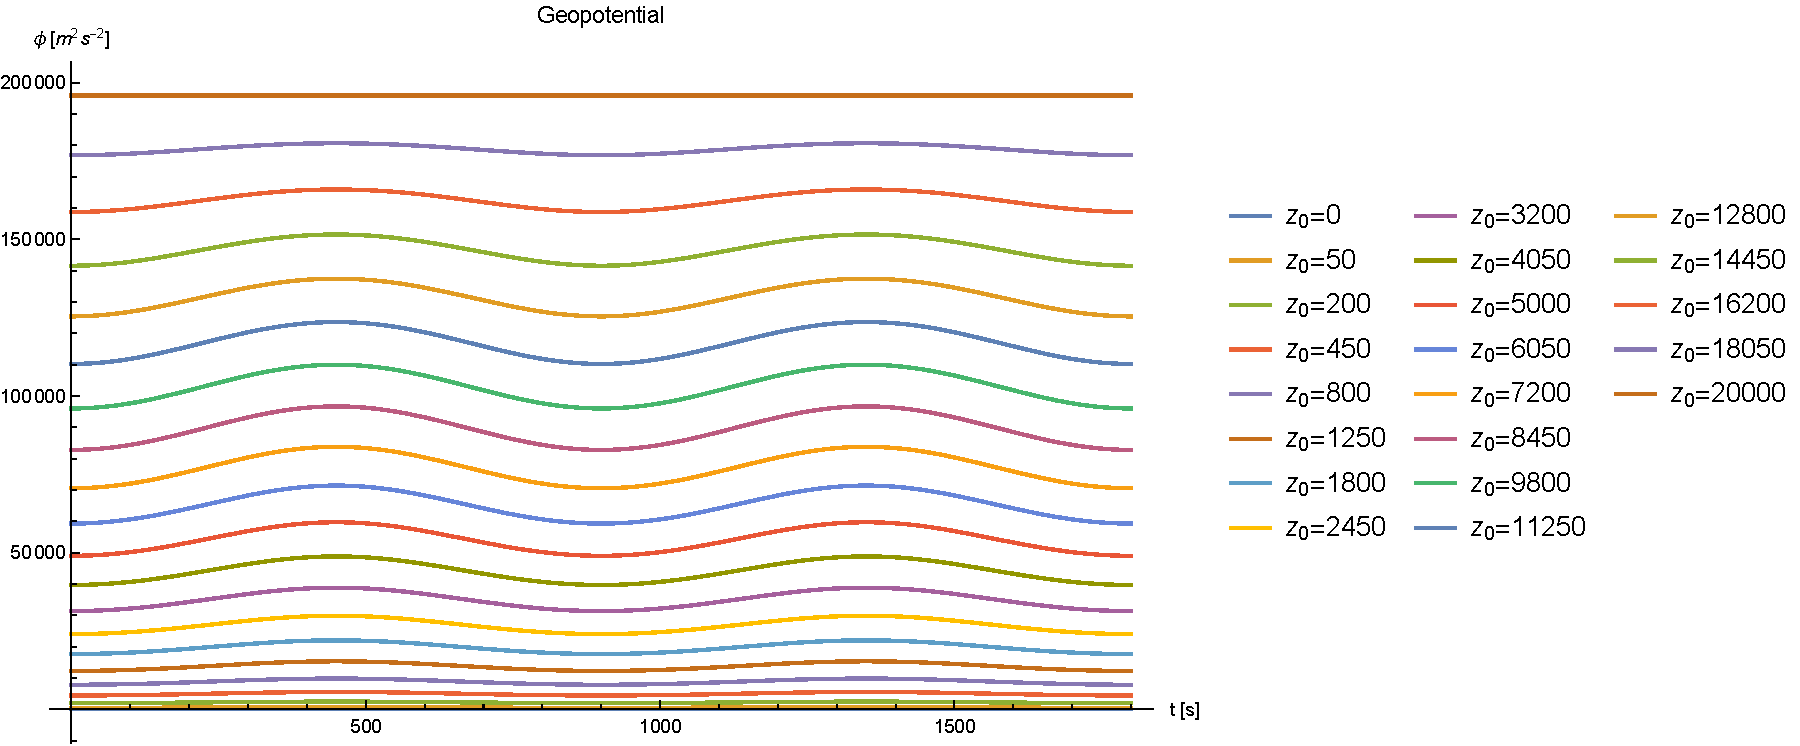
\includegraphics[width=\linewidth]{figures/geopotential_plot}
  \caption{Geopotential $\phi(t)$ for $\phi_0 = gz_0$ and $z_0$ values listed in the legend, with parameters $w_0=5$, $T_{v0}=300$, $\Gamma_v=0.01$, $z_{top}=20000$, $t_p=900$.}\label{fig:geopotential}
\end{figure}

We use \eqref{eq:phi_vel} to find the divergence, which is required by the continuity equation \eqref{eq:continuity},
\begin{equation}\label{eq:div}
  \partd{w}{\phi}(\phi,t) = \frac{\pi w_0}{g z_{top}}\cos\frac{\pi \phi(t)}{gz_{top}}\sin\frac{2\pi t}{t_p}.
\end{equation}
Substituting \eqref{eq:div} into \eqref{eq:continuity}, we find another separable ODE:
\begin{align*}
  \deriv{\rho}{t} &= -\rho \left(\frac{\pi w_0}{z_{top}}\cos\frac{\pi \phi(t)}{g z_{top}}\sin\frac{2\pi t}{t_p}\right)\\
  \Rightarrow \int \frac{1}{\rho}\,d\rho &= -\frac{\pi w_0}{z_{top}}\cos\frac{\pi \phi(t)}{z_{top}}\int \sin \frac{2\pi t}{t_p}\,dt.
\end{align*}
The solution is
\begin{align}\label{eq:density}
  \rho(\phi(t),t) = \rho_0(\phi_0)\exp\left[\frac{ w_0 t_p}{2z_{top}}\left(\cos\frac{\pi {\phi}(t)}{gz_{top}}\cos\frac{2\pi t}{t_p}-\cos\frac{\pi {\phi_0}}{gz_{top}}\right)\right].
\end{align} 

\begin{figure}[H]
  \centering
  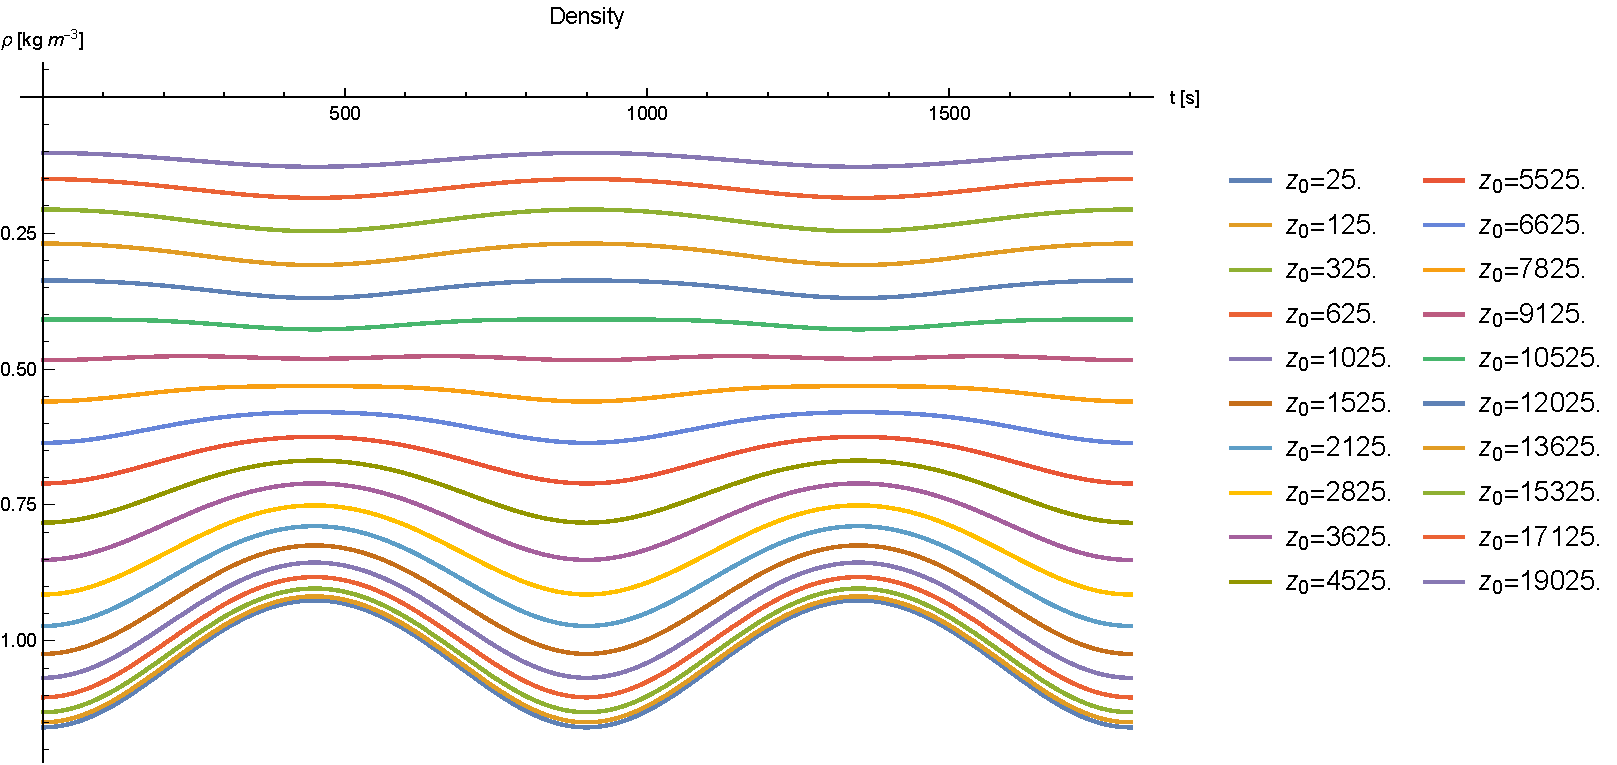
\includegraphics[width=\linewidth]{figures/density_plot}
  \caption{Density $\rho(\phi(t),t)$ for $\phi_0 = gz_0$ and $z_0$ values listed in the legend, with parameters $w_0=5$, $T_{v0}=300$, $\Gamma_v=0.01$, $z_{top}=20000$, $t_p=900$.}\label{fig:density}
\end{figure}

To find the pressure, we use \eqref{eq:density} in \eqref{eq:eos},
\begin{align}
  \frac{p}{\Pi} &= R\rho(\phi(t),t)\theta_v(\phi(t),t),\notag \\
  p(\phi(t),t) &= \left(p_{ref}^{-\kappa} R \rho(\phi(t),t)\theta_v(\phi(t),t)\right)^{1/(1-\kappa)}.\label{eq:pressure}
\end{align}

\begin{figure}[H]
  \centering
  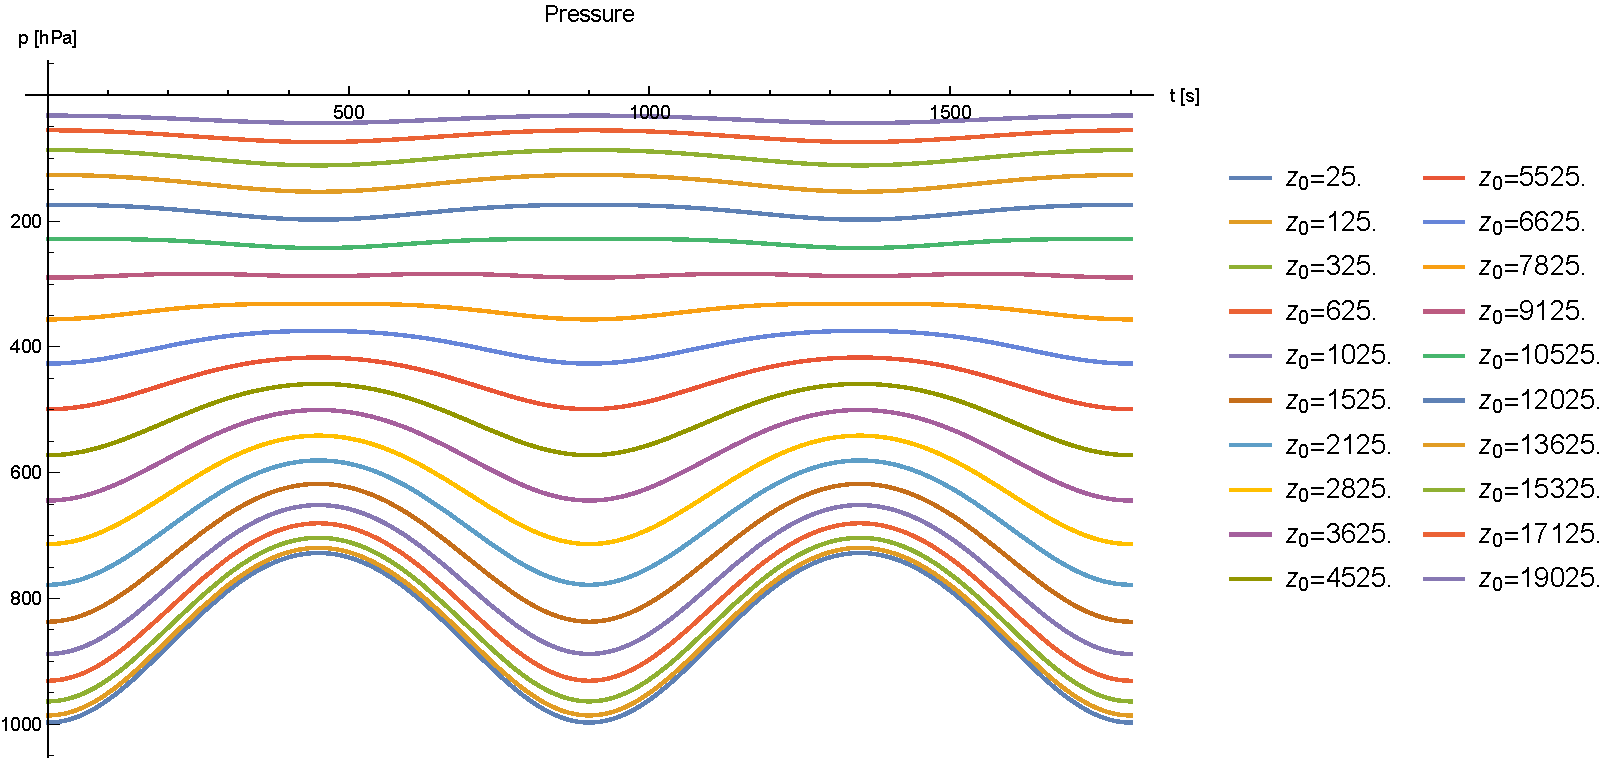
\includegraphics[width=\linewidth]{figures/pressure_plot}
  \caption{Pressure $p(\phi(t),t)$ for $\phi_0 = gz_0$ and $z_0$ values listed in the legend, with parameters $w_0=5$, $T_{v0}=300$, $\Gamma_v=0.01$, $z_{top}=20000$, $t_p=900$.}\label{fig:pressure}
\end{figure}

\subsection{Physical interpretation}

Physically, the ansatz \eqref{eq:z_vel} may be interpreted via \eqref{eq:momentum} as defining the balance between buoyancy, the pressure gradient force, and gravity to be,
\begin{align}
  -g\left(1 +  \frac{1}{\rho}\partd{p}{\phi}\right) &= \deriv{w}{t}(\phi,t), \notag \\
  &= \frac{2\pi w_0}{t_p}\sin\frac{\pi\phi}{gz_{top}}\cos\frac{2\pi t}{t_p} + \frac{\pi w_0^2}{2z_{top}}\sin\frac{2\pi\phi}{gz_{top}}\sin^2\frac{2\pi t}{t_p},
\end{align}
where the right-hand side is the time derivative of \eqref{eq:phi_vel}.
It is most straightforward to derive this interpretation by decomposing the pressure into a constant, hydrostatically balanced reference state with a superimposed perturbation \cite{KlempWilhelmson1978,Srivastava1967,SoongOgura1973} so that $p = \overline{p} + p'$.
Combining this decomposition (and similar treatment of temperature and density) with the equation of state leads to a formulation of the total pressure gradient as the background hydrostatic balance plus a perturbation due to nonhydrostatic buoyancy.  
In \cite{KlempWilhelmson1978,Srivastava1967,SoongOgura1973} this arises as quadratic terms of the perturbation variables are neglected.  
It is interesting that a similar (though not equivalent\footnote{Taylor et.~al.~\cite{Taylor2020} retain the full form of the pressure gradient, without a linearization.}) term arises in \cite{Taylor2020} as a result of the choice of a vertical mass coordinate based on hydrostatic pressure.
  
\subsection{Initialization}

Initial conditions are defined by stationary, $w(\phi(0),0) = 0,$ hydrostatic balance with a constant lapse rate in the virtual temperature profile, and exponential decay in the water vapor mixing ratio.

The initial virtual temperature profile is defined by two parameters, $T_{0}$ and $\Gamma_v$ (with default values 300K and 0.01 K/m, respectively),
\begin{equation}\label{eq:tv}
  T_{v0}(z) = T_{0} - \Gamma_v z.
\end{equation}
Using \eqref{eq:tv} with $p=\rho R T_v$, an equivalent form of the equation of state \eqref{eq:eos}, the hydrostatic equation $\partd{p}{z} = -\rho g$, and separation of variables (again), we derive expressions that relate initial height to initial pressure,
\begin{align}
  p_0(z) = \begin{cases}
          p_{ref}\exp\left(\frac{-g z}{R T_{0}}\right) & \Gamma_v = 0,\\[0.5em]
          p_{ref}\, T_0^{-g/(R\Gamma_v)}\left(T_{0} - \Gamma_v z\right)^{g/(R\Gamma_v)} & \Gamma_v \ne 0,
        \end{cases} \label{eq:p_of_z}\\[0.5em]
  z_0(p) = \begin{cases}
         -\frac{R T_{0}}{g}\log\frac{p}{p_{ref}} & \Gamma_v = 0,\\[0.5em]
         \frac{T_{0}}{\Gamma_v}\left(1 - \left(\frac{p}{p_{ref}}\right)^{R\Gamma_v/g}\right) & \Gamma \ne 0.
       \end{cases}\label{eq:z_of_p}
\end{align}
It follows that the initial virtual potential temperature profile is defined as
\begin{equation}
  \theta_{v0}(z) = T_{v0}(z)\left(\frac{p_{ref}}{p_0(z)}\right)^\kappa.
\end{equation}
The initial water vapor mixing ratio profile is also defined by two parameters, $q_0$ and $q_1$, with default values $q_0=0.015$ kg H$_2$O / kg air and $q_1 = $ 1E-3 m$^{-1}$, as
\begin{equation}\label{eq:init_qv}
  q_{v0}(z) = q_0e^{-q_1 z}.
\end{equation}
Initial densities are defined as
\begin{equation}
  \rho_0(z) = \frac{p_0(z)}{R\,T_{v0}(z)}.
\end{equation}

\subsection{Discretized column}

The Haero column is defined by first setting the required parameters using the \texttt{haero::driver::AtmosphericConditions} class.
These include the model top $z_{top}$, maximum vertical velocity $w_0$, and velocity period $t_p$ in \eqref{eq:phi_vel}, the initial virtual temperature profile \eqref{eq:tv}, and the initial water vapor mixing ratio profile \eqref{eq:init_qv}.

In the Haero driver, we emulate the vertical grid staggering used by the HOMME-NH dynamical core \cite{Taylor2020}, which has $n_{lev}$ levels and $n_{lev}+1$ interfaces.
Levels are indexed by integer values $k$, for $k=1,\dotsc,n_{lev}$ and interfaces are indexed by $k+1/2$, for $k=0,\dotsc,n_{lev}$.

In the \texttt{haero::driver::HostDynamics} class, geopotential and vertical velocity are defined at interfaces;
\begin{align}
  \phi_{k+1/2}(t) &= \frac{2gz_{top}}{\pi}\arctan\left[\tan\frac{\pi \phi_{k+1/2}(0)}{2g z_{top}}\exp\left(\frac{w_0t_p}{2z_{top}} \sin^2 \frac{2\pi t}{t_p}\right)\right], \label{eq:phi_disc}\\
  w_{k+1/2}(t) &= w_0 \sin \frac{\pi \phi_{k+1/2}(t)}{g z_{top}}\sin\frac{2\pi t}{t_p}. \label{eq:w_disc}
\end{align}
Similarly, density, virtual potential temperature, water vapor, and pressure are defined at level midpoints,
\begin{align}
  \rho_k(t) &= \rho_0(\overline{\phi_k}(0))\exp\left[\frac{ w_0 t_p}{2z_{top}}\left(\cos\frac{\pi \overline{\phi_k}(t)}{gz_{top}}\cos\frac{2\pi t}{t_p}-\cos\frac{\pi \overline{\phi_{k}}(0)}{gz_{top}}\right)\right], \label{eq:rho_disc}\\
  \theta_{vk}(t) &= \theta_{v0}(\overline{\phi_k}(0)/g), \label{eq:thetav_disc} \\
  q_{vk}(t) &= q_{v0}(\overline{\phi_k}(0)/g), \label{eq:qv_disc} \\
  % p_k(t) &= \left(p_0^{-\kappa}R \, \rho_k(t)\,\left(\theta_v\right)_k(t)\right)^{1/(1-\kappa)}, 
p_k(t) &=  \left(p_{ref}^{-\kappa} R \rho_k(t)\theta_{vk}(t)\right)^{1/(1-\kappa)}\label{eq:p_disc}
\end{align}
where the constants $g = 9.8$ m/s$^2$, $p_{ref} = 10^5$ Pa, and $\kappa = 0.286$; the overline denotes an average, $\overline{\phi_k}(t) = (\phi_{k-1/2}(t) + \phi_{k+1/2}(t))/2$.

Users may opt to initialize a column with uniform spacing in either height or pressure (at interfaces), or to specify their own height or pressure interfaces via an input \texttt{.yaml} file.  
The model top is defined by \eqref{eq:z_of_p}.  

Unit tests verify the expected 2nd order convergence of the centered finite difference methods used by both HOMME-NH and the Haero driver, and that layer thicknesses sum to the correct values $z_{top}$ and $p_{top}$, as shown in Figure \ref{fig:fd_verification}.

\begin{figure}[H]
\centering 
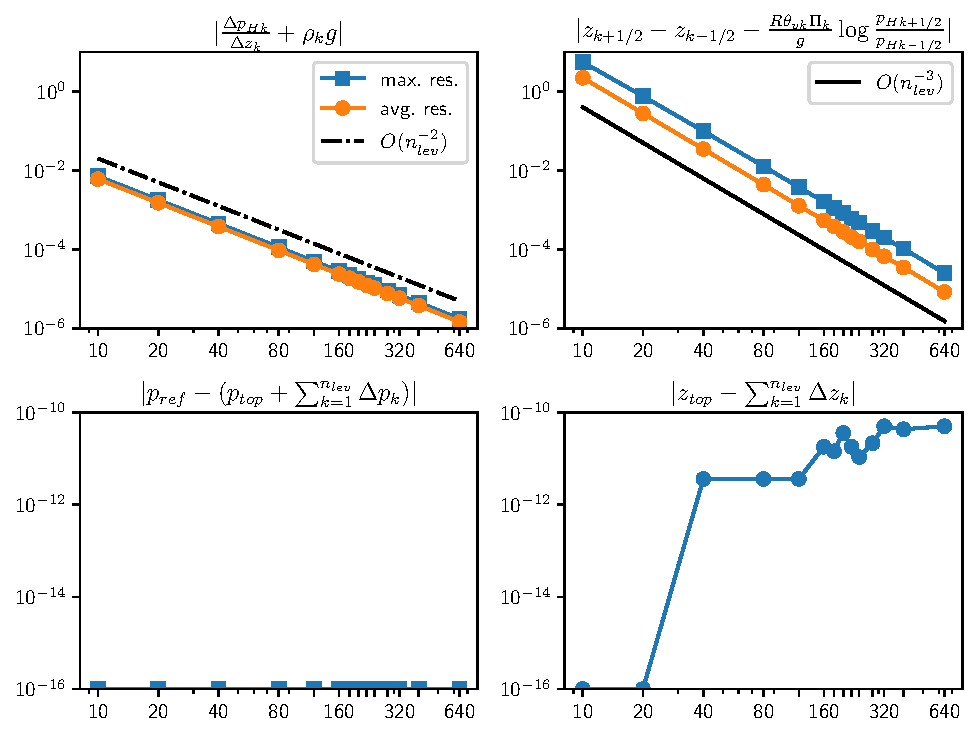
\includegraphics[width=0.8\linewidth]{figures/vconv_plot}
\caption{Vertical finite difference verification. Clockwise from top left: hydrostatic balance, hypsometric layer thickness, sum of height thicknesses, sum of pressure thicknesses.}\label{fig:fd_verification}
\end{figure}

\subsubsection{Layer thickness}

Layer thickness in height units is computed directly as 
\begin{equation}\label{eq:z_thick}
  \Delta z_k = \left(\phi_{k-1/2} - \phi_{k+1/2}\right)/g,
\end{equation}
which reflects the true thickness of a model level in our non-hydrostatic model.
However, some legacy parameterizations require thickness defined in \emph{pressure} units.
To support these parameterizations, we compute \texttt{hydrostatic\_dp} as a member of the \texttt{HostDynamics} class.
This calculation begins by defining the hydrostatic pressure $p_H$ at each interface, $p_{H,k+1/2} = p(\phi_{k+1/2}/g)$ using \eqref{eq:z_of_p}.
Then the layer thickness is computed as
\begin{equation}\label{eq:p_thick}
  \Delta p_{Hk} = p_{H,k+1/2} - p_{H,k-1/2}.
\end{equation}
\begin{assume}[Hyrdostatic layer thickness]
  Pressure thickness is computed via the hydrostatic approximation.  
\end{assume}

The interface hydrostatic pressures $p_H$ are stored as a private variable, to prevent users from mistaking them for the full non-hydrostatic pressure.

\subsection{Creating a Haero atmosphere}

The above dynamics are motivated by the input requirements of the various parameterizations.  
These are encapsulated by the \texttt{haero::Atmosphere} class, which requires temperature, pressure, height, and relative humidity data. 
We already have pressure and height.
Temperature may be diagnosed using the approximation given by \cite[eq.~(2.3)]{KlempWilhelmson1978},
\begin{equation}\label{eq:approx_temp}
  T_k(t) \approx \frac{\theta_{vk}(t) ~ \Pi_k(t)}{1+\alpha_q ~ q_{vk}(t)},
\end{equation}
with constant $\alpha_q = 0.61$.

\begin{figure}[H]
  \centering
  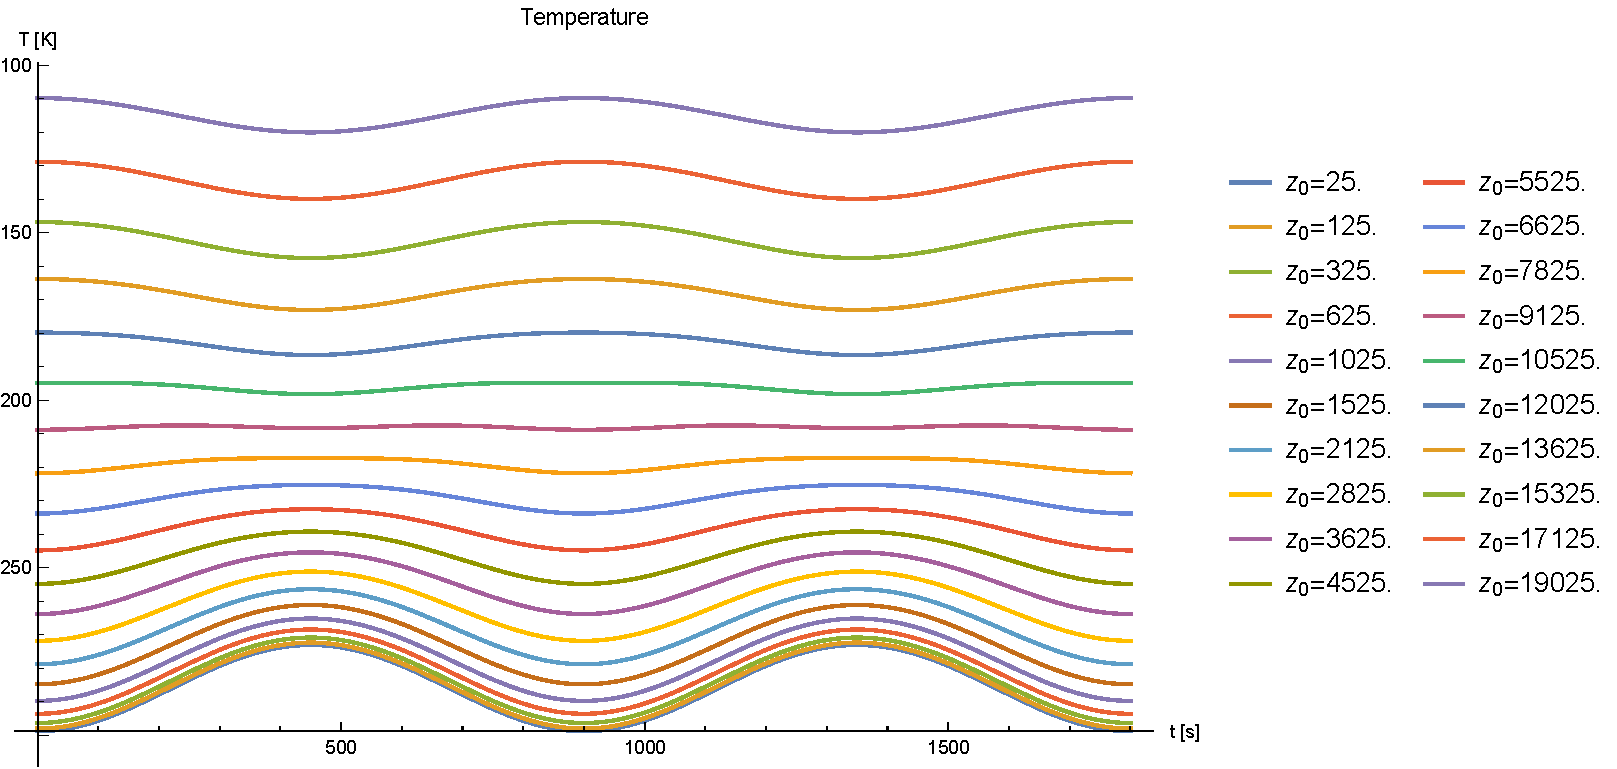
\includegraphics[width=\linewidth]{figures/temperature_plot}
  \caption{Temperature for the same parameters as in Figures \ref{fig:geopotential},\ref{fig:density}, and \ref{fig:pressure}, with the additional parameters $q_{0}=6$E-3, $q_1=2.5$E-3.}\label{fig:temperature}
\end{figure}

We compute relative humidity as $s = q_v/q_{vsat}$, where $q_{vsat}$ is the saturation mixing ratio.
We use the Tetens equation to find $q_{vsat}$ \cite[eqn. (A1)]{SoongOgura1973},
\begin{equation}\label{eq:tetens}
  q_{vs}(T) = \frac{380.042}{p}\exp\left(\frac{15}{2}\log(10) \frac{T-273}{T-36}\right).
\end{equation}

\begin{figure}[H]
\centering
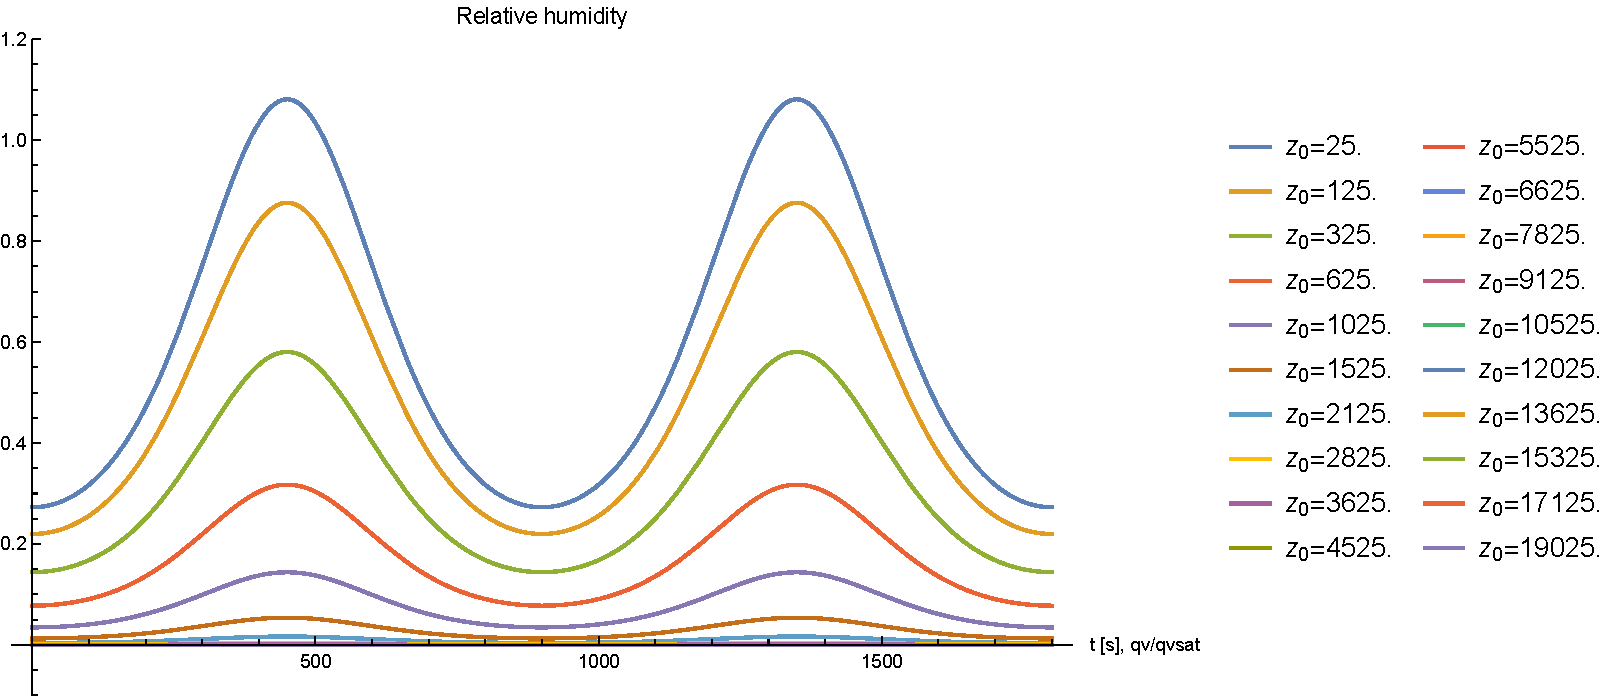
\includegraphics[width=\linewidth]{figures/relhumidity_plot}
\caption{Temperature for the same parameters as in Figures \ref{fig:geopotential},\ref{fig:density}, and \ref{fig:pressure}, with the additional parameters $q_{0}=6$E-3, $q_1=2.5$E-3.}\label{fig:humidity}
\end{figure}


\subsection{Time stepping}

The above dynamics are associated with the following \emph{tendencies}, the right-hand sides of \eqref{eq:geo_traj} and \eqref{eq:1d},
\begin{subequations}\label{eq:tends}
  \begin{align}
     \dot{w}(\phi,t) \equiv \totd{w}  &= \frac{2\pi w_0}{t_p}\sin\frac{\pi\phi}{gz_{top}}\cos\frac{2\pi t}{t_p} + \frac{\pi w_0^2}{2z_{top}}\sin\frac{2\pi\phi}{gz_{top}}\sin^2\frac{2\pi t}{t_p},\\
    \dot{\phi}(\phi,t) \equiv \totd{\phi} &= gw_0 \sin \frac{\pi \phi}{g z_{top}}\sin\frac{2\pi t}{t_p},\\
    \dot{\rho}(\phi, t, \rho) \equiv \totd{\rho} &= -\rho \frac{\pi w_0}{z_{top}}\cos\frac{\pi \phi}{g z_{top}}\sin\frac{2\pi t}{t_p},\\
    \dot{\theta_v} \equiv \totd{\theta_v} &= 0,\\
    \dot{q_v} \equiv \totd{q_v} &= 0,
  \end{align}
\end{subequations} 
where the dot denotes differentiation with respect to time.

\subsubsection{Simple microphysics}

A simple cloud model with warm-rain microphysics, often called \emph{Kessler microphysics}, is summarized in \cite[ch.~15]{RogersYau}, which references \cite{Srivastava1967}.
It introduces mass mixing ratio tracers for cloud liquid water $q_c$ and rain water $q_r$ and source terms for the dynamics equations.  
We use \cite{SoongOgura1973,KlempWilhelmson1978} as additional references.
We adapt this microphysics model here to match the HOMME-NH dynamics variables.

The two new tracers are advected passively by the dynamics (without source and sink terms) in the same manner as water vapor,
\begin{subequations}
  \begin{align}
    \dot{q_c} \equiv \deriv{q_c}{t} &= 0,\\
    \dot{q_r} \equiv \deriv{q_r}{t} &= 0.
  \end{align}
\end{subequations}
Microphysical parameterizations define approximate source and sink terms to correspond to a select (incomplete) set of physical processes, as described below.


\paragraph{Vertical velocity.} The vertical velocity $w$ is adjusted to account for loss of buoyancy due to the mass of suspended liquid water, 
\begin{equation*}
  \dot{w} \pluseq -g(q_c+q_r).  
\end{equation*}

\paragraph{Evaporation and condensation.}

Our first step assumes unsaturated air, $q_v \le q_{vs}$, where $q_{vs}$ is the saturation mixing ratio defined by \eqref{eq:tetens} using the temperature computed by \eqref{eq:approx_temp},
\begin{subequations}\label{eq:evap}
  \begin{align}
    \dot{q_v} &\pluseq E_{cv} + E_{rv}, \\
    \dot{q_c} &\minuseq E_{cv}, \\
    \dot{q_r} &\minuseq E_{rv},  \\
    \dot{\theta_v} &\minuseq \frac{L}{c_p \Pi}(E_{cv} + E_{rv}),
  \end{align}
where $E_{cv}$ and $E_{rv}$ denote the evaporation rates between cloud liquid/water vapor and rain/water vapor, respectively.
\begin{equation}\label{eq:cloud2vapor_evap}
   E_{cv} = \begin{cases} q_c & \text{if } q_v < q_{vs} \\ 0 & \text{otherwise}\end{cases}
\end{equation}
\begin{equation}
  E_{rv} = \begin{cases} \frac{(1-q_v/q_{vs}) C_{vt} (\rho q_r)^{0.525}}{\rho 5.4\text{E}5 + 4.1\text{E}6/e_s(T)} & \text{if } q_v < q_{vs} \text{ and } q_c = 0 \\ 0 & \text{otherwise}\end{cases}
\end{equation}
The ventillation coefficient $C_{vt} = 1.6 + 5.7\text{E-}2V_r^{3/2}$ for rain falling at speed $V_r$ relative to the air, and $e_s(T)$ is the saturation vapor pressure for a planar liquid water surface at temperature $T$.  
The latter two values are approximated as \cite[eqn.~(15))]{SoongOgura1973},
  \begin{align}
    V_r & = 36.34 (1\text{E}3\rho q_r)^{0.1364} \text{ m/s},\\
    e_s(T) & = 6.1094\exp\left( \frac{17.625 (T-273)}{T-29.96} \right)\text{ hPa}.
  \end{align}
\end{subequations}
\textbf{Note:} The exponent 0.1364 in the fall velocity expression is as written in \cite[eqn. (15)]{SoongOgura1973}; in  \cite[eqn.~(2.15)]{KlempWilhelmson1978} it's written as 0.1346.  
The authors of \cite{KlempWilhelmson1978} modify the expression used in \cite{SoongOgura1973} to include a reference density term (and make a similar modification to the ventilation coefficient). 
Since this modification is unrelated to the exponent, we have assumed that 0.1346 is a typographical error and we use the value from \cite{SoongOgura1973} in this work.

A second step \cite[eqns.(A7)--(A10)]{SoongOgura1973} conducts an adjustment for supersaturated air, $q_v > q_{vs}$, after the time stepping procedure implied by \eqref{eq:evap} is finished.
Let these values be denoted by a star: $\theta_v^*$, $q_v^*$, $q_c^*$, etc. 
\begin{subequations}
Define the factor $r_1$,
\begin{equation}
  r_1 = \left(1 + \frac{237 a\Pi q_{vs}^*}{(T^*-36)^2}\frac{L}{c_p\Pi} \right)^{-1}.
\end{equation}
Then the adjusted values are given as
\begin{align}
  q_v &= q_{v}^* - r_1(q_v^*-q_{vs}^*),\\
  \theta_v & = \left(\theta^* + \frac{Lr_1}{c_p\Pi}(q_v^*-q_{vs}^*)\right)\left(1 + \alpha_v q_v\right),\\
  q_c &= q_v^* + q_c^* - q_v.
\end{align}
\end{subequations}


\paragraph{Autoconversion.} Autoconversion of cloud liquid into rain only occurs in the presence of sufficient cloud water droplets.
Here, ``sufficient'' is defined as greater than a constant critical value, $q_c^{(crit)}$, and \cite[eqn.~(12)]{Srivastava1967}
\begin{subequations} \label{eq:autoconversion}
\begin{align}
  \dot{q_c} &\minuseq \alpha_{auto}(q_c - q_c^{(crit)})_+,\\
  \dot{q_r} &\pluseq \alpha_{auto}(q_c - q_c^{(crit)})_+,
\end{align}
\end{subequations}
where $\alpha_{auto}$ [1/s] is the inverse of the autoconversion time scale and $q_c^{(crit)}$ is a user-defined parameter.
In \cite{SoongOgura1973}, $\alpha_{auto}=1\text{E-3}$ s$^{-1}$ and $q_c^{(crit)} = 1\text{E-3}$.

\paragraph{Accretion.} Accretion describes the capture of cloud water droplets by rainwater droplets.
As in \cite{SoongOgura1973,KlempWilhelmson1978}, we use
\begin{subequations}\label{eq:accretion}
\begin{align}
  \dot{q_c} &\minuseq \alpha_{accr}q_cq_r^{7/8}, \\
  \dot{q_r} &\pluseq \alpha_{accr} q_c q_r^{7/8},
\end{align}
\end{subequations}
with $\alpha_{accr} = 2.2$.

\paragraph{Rainwater sedimentation.} 

\begin{equation}
  \dot{q_r} \minuseq \frac{1}{\rho}\partd{}{z}(\rho V_rq_r)
\end{equation}

At the model top, this term is zero.

\todo{lower boundary}

\paragraph{Turbulent mixing.}

We modify sub-grid scale turbulence mode of \cite{KlempWilhelmson1978} to use a simple Smagorinsky turbulent eddy mixing coefficient,
\begin{equation}
  K_m = \sqrt{2}\left(\frac{7l}{50}\right)^2 \abs{\partd{w}{z}}.
\end{equation}
The additional source terms are \cite[eqns.~(3.15)--(3.16)]{KlempWilhelmson1978}
\begin{align}
  \dot{w} &\pluseq 2 \partd{}{z}\left(K_m \partd{w}{z}\right) - \frac{20}{3 l^2}K_m\partd{K_m}{z},\\
  \dot{q_v} &\pluseq 3\partd{}{z}\left(K_m\partd{q_v}{z}\right), \\
  \dot{q_c} &\pluseq 3\partd{}{z}\left(K_m\partd{q_c}{z}\right), \\
  \dot{\theta} &\pluseq 3\partd{}{z}\left(K_m\partd{\theta}{z}\right). 
\end{align}
\todo{Boundary conditions}
\subsection{Embedded parameterization}


\appendix
\chapter{Glossary}
\labelappendix{glossary}

This section contains definitions of important terms and mathematical quantities
used in Haero.

\section{Terminology}
\labelappendixsection{terminology}

\begin{itemize}
  \item Cloud Condensation Nuclei (CCN):
  \item Precursors:
  \item Secondary Aerosols:
\end{itemize}

\section{Mathematical Notation}
\labelappendixsection{notation}

The following symbols are used in equations within Haero's aerosol processes.
Relevant units are given in square brackets next to their symbols. [-] indicates
that a quantity is unitless.

\begin{itemize}
  \item $T$ [K]: air temperature

  \item $p$ [Pa]: air pressure

  \item $\specidx$: index of chemical species

  \item $\mw{\specidx}$ [kg/kmol]: molecular weight of species $\specidx$

  \item $\mathscr{R}$ [J/kmol/K]: universal gas constant

  \item $R_{\specidx}$ [J/kg/K]: gas constant specific to species $\specidx$:
        $R_{\specidx} = \mathscr{R}/\mw{\specidx}$

  \item $c\dsub{air}$ [kmol air / m$^3$ air]: molar concentration of dry air:
    \begin{equation}
      c\dsub{air} = \frac{p}{\mathscr{R}T} = \frac{\rho\dsub{air}}{M\dsub{air}}
    \end{equation}
    where $\rho\dsub{air}$ and $M\dsub{air}$ are the density and molecular weight
    of dry air, respectively. Note that
    $M\dsub{air} = 28.966$~kg~$\cdot$~kmol$^{-1}$ in E3SM.

  \item $\rho\dsub{\specidx}$ [kg/m$^3$]: density of species $\specidx$
        (gas, liquid or solid)
    \hwc{For liquid- and solid-phase species there seems to be two types of
      densities:
      \begin{enumerate}
        \item mass divided by the volume of air in which they are suspended
        \item mass divided by the volume the liquid or solid matter occupies
      \end{enumerate}
      $\rho\dsub{\specidx}$ seems to be fall in to the first type. Let's watch
      out for places of potential confusion.}

  \item $i$, $j$: indices of log-normal modes

  \item $I$: total number of log-normal modes

  \item $D\dsub{p}$: particle diameter, unit: $\rm m$

  \hwc{Which of the following notations need to be distinguished for
       interstitial and cloud-born aerosols?}
  \jsc{We at least need different notations for interstitial and cloud-borne
       aerosols for $\amass{\specidx}$ and $q\dsub{n,i}$ in the rename process.
       All the other parameters are related to $\amass{\specidx}$ and
       $q\dsub{n,i}$ so we may also need to use different notation.}

  \item $N\dsub{i}$ [\#/m$^{-3}$]: number concentration of particles in mode $i$

  \item $n\dsub{i} (D\dsub{p})$ [m$^{-4}$]: size distribution of aerosol
        particles in mode $i$, expressed as a function of $D\dsub{p}$
        (\refeq{n_Dp})

  \item $n\dsub{i} (\ln D\dsub{p})$ [m$^{-3}$]: size distribution of aerosol
        particles in mode $i$, expressed as a function of $\ln D\dsub{p}$
        (\refeq{n_lnDp})

  \item $n\dsub{norm,i} (\ln D\dsub{p})$ [-]: $n\dsub{i} (\ln D\dsub{p})$
        normalized by the mode's number concentration $N\dsub{i}$

  \item $D\dsub{gn,d,i}$ [m]: geometric mean of dry particle diameter
        $D\dsub{p}$ in mode $i$

  \item $D\dsub{gn,w,i}$ [m]: geometric mean of wet particle diameter
        $D\dsub{p}$ in mode $i$

  \item $\sigma\dsub{g,i}$ [-]: geometric standard deviation of $D\dsub{p}$ in
        mode $i$
        \hwc{Why is it unitless?}
        \jsc{The unit of $\sigma\dsub{g,i}$ should be the same as that of
             $D\dsub{p}$. $\ln D\dsub{p}$ and $\ln \sigma\dsub{g,i}$ are
             unitless. According to Seinfeld's book, when we write
             $\ln D\dsub{p}$ and $\ln \sigma\dsub{g,i}$, we really mean
             $\ln \frac{D\dsub{p}}{1}$ and $\ln \frac{\sigma\dsub{g,i}}{1}$,
             where 1 is the ``reference'' particle diameter or standard
             deviation and not explicitly indicated.}

  \item $V\dsub{d,i}$ [m$^3$ particles/m$^3$ dry air]: volume concentration of
        dry aerosol particles in mode $i$

  \item $V\dsub{w,i}$ [m$^3$ particles/m$^3$ dry air]: volume concentration of
        wet aerosol particles in mode $i$

  \item $V\dsub{\specidx,i}$ [m$^3$ species $\specidx$/m$^3$ dry air]: dry
        volume of species $\specidx$ in mode $i$

  \item $q\dsub{n,i}$ [\#/kmol]: total number mixing ratio of particles in mode
        $i$

  \item $\amass{\specidx}$ [kmol species $\specidx$/kmol dry air] in microphysics,
        [kg species $\specidx$/kg dry air] in dry/wet deposition: mass mixing
        ratio for aerosol species $\specidx$ in mode $i$
        % listed in Section~\ref{sec:MAM_procs_and_eqns})

  \item $\rho\dsub{d,i}$ [kg dry aerosol particles/m$^3$ dry aerosol particles]:
        density of dry aerosol particles in mode $i$

  \item $\rho\dsub{w,i}$ [kg of wet aerosol particles/m$^3$ wet aerosol
        particles]: density of wet aerosol particles in mode $i$

  \item $\vmass{\specidx}$ [kmol species $\specidx$/kmol dry air] in microphysics,
        [kg species $\specidx$/kg dry air] in other parameterizations: mass
        mixing ratio for gas species (vapor)

  \item $\Delta t\dsub{phys}$ [s]: time step size for aerosol physics
\end{itemize}

\section{The MAM Application Programming Interface}
\labelappendix{api}


\include{process_appendix}
\chapter{Driver Input Specification}
\labelappendix{driver_input}

Below is the input specification for the Haero driver. The spec uses
[YAML](https://yaml.org/). Compared to Fortran namelists, YAML offers

\begin{itemize}
  \item {\bf better readability}: YAML files are flexible, and don't have a lot
    of "kibble" (braces, tags, and other stuff you see routinely in fancier
    markup like XML, HTML, and so on). They're very easy to read.
  \item {\bf better validation}: YAML files have named entries that can be
    used or ignored, depending on the needs of the particular application.
    Also, the file format allows for error checking.
  \item {\bf better language support}: Fortran namelists are so-called because
    they are only available to Fortran. YAML has libraries that allows it to
    be used with several programming languages (including Fortran!). This makes
    it easier for tools and other applications to use similar input files. In
    particular, this allows workflows to use a single input file to define a
    workload that can be processed with several tools.
  \item {\bf support for lists and maps}: YAML offers constructions for
    dynamically-sized datasets. Haero focuses on runtime configurability,
    so the ability to add species (and perhaps even modes) to an input file
    is important.
  \item {\bf a larger support community}: Fortran remains a niche language,
    which often instills a sense of pride in scientists. Unfortunately, the
    downside to belonging to a small community of specialists is that the tools
    are invariably of lower quality than more commonly-used tools. One needs
    only to witness the notorious ongoing issues with Fortran compilers to see
    this phenomenon firsthand.
\end{itemize}

This specification is for use only with the Haero driver. The library provides
no input/output interface---it assumes that the model in which it's embedded
does the work of assembling input data and loading it into the appropriate
data structures.

The Haero driver is a single-column aerosol dynamics simulator---it doesn not
model horizontal dynamics. However, depending on how initial conditions are
specified, it's possible to generate ensembles whose members are individual
atmospheric columns. Because the columns are independent of one another, these
ensembles can be run entirely within a single simulation, allowing the driver
to take advantage of parallelism, and allowing statistics and measures of
convergence to be generated.

\subsection*{Sections}

A YAML file consists of several named sections. Each of these sections can
contain data and metadata. Sections are a powerful tool for organizing input
using simple concepts with human-readable notation.

\subsubsection*{Modes}

The \texttt{modes} section defines the particle size modes available to a Haero
model. As we discussed in \refsubsection{lib:modes}, a mode has metadata
specifying its size range and its geometric standard deviation.

\begin{verbatim}
modes:
  aitken:
    D_min: 0.0087
    D_max: 0.052
    sigma: 1.6
  accumulation:
    D_min: 0.0535
    D_max: 0.44
    sigma: 1.8
  coarse:
    D_min: 1.0
    D_max: 4.0
    sigma: 1.8
  primary_carbon:
    D_min: 0.01
    D_max: 0.1
    sigma: 1.6
\end{verbatim}

Particle diameters and $\sigma$ are measured in $\mu\mathrm{m}$.

The \texttt{modes} section is essentially a map whose keys are mode names
(\texttt{aitken}, \texttt{accumulation}, \texttt{coarse}, and \texttt{primary\_carbon},
in the example above), and whose values are themselves maps. The map for a given
mode contains the following fields:

\begin{itemize}
  \item \texttt{D\_min}: the minimum diameter of particles belonging to the mode
  \item \texttt{D\_max}: the maximum diameter of particles belonging to the mode
  \item \texttt{sigma}: the geometric mean standard deviation for the size
                        distribution for particles belonging to the mode
\end{itemize}

Everything in a mode must be completely specified---there are no default values.

\subsubsection*{Aerosol Species}

Aerosol species populate each of the defined modes, and are defined in the
\texttt{aerosols} section. As we discussed in \refsubsection{lib:species}, a
species is defined by its elemental composition and its electric charge (given
in units of the electronic charge $|e|$).
%The \texttt{species} section follows the same format as defined by
%\href{https://cantera.org/documentation/dev/sphinx/html/yaml/species.html}{Cantera}.

Like the \texttt{modes} section, the \texttt{aerosols} section is a map whose keys
are {\em symbolic names} of aerosol particle species (e.g. \texttt{SO4} for
sulfate particles):

\begin{verbatim}
aerosols:
  SO4:
    name: sulfate
  NH4:
    name: ammonium
  POA:
    name: primary organic aerosol
  SOA:
    name: secondary organic aerosol
  BC:
    name: black carbon
  SS:
    name: sea salt
  DST:
    name: dust
  MOA:
    name: marine organic aerosol
\end{verbatim}

An aerosol species has the following fields:

\begin{itemize}
  \item \texttt{name}: the full name for the species (e.g. \texttt{sulfate} for
    \texttt{SO4}). You don't need to quote the full name, even if it contains
    spaces.
\end{itemize}

\subsubsection*{Gas Species}

Gas species exist in the atmosphere, and aren't associated with modes. These
species are defined in the \texttt{gases} section.

The \texttt{gases} section is identical in structure to the
\texttt{aerosols} section:

\begin{verbatim}
gases:
  SO2:
    name: sulfur dioxide
  H2SO4:
    name: sulfuric acid
  SOAG:
    name: single semi-volatile organic gas-phase species
  NH3:
    name: ammonia
\end{verbatim}

A gas species has the following fields:

\begin{itemize}
  \item \texttt{name}: the full name for a gas species (e.g.
    \texttt{sulfur dioxide} for \texttt{SO4}. You don't need to quote the
                     full name, even if it contains spaces.
\end{itemize}

\subsubsection*{Physics}

In this section, we tell the Haero driver what physical processes we wish
to simulate. Every field in this section assumes a \texttt{true} or
\texttt{false} value, so it's really just a set of ON/OFF switches. Valid fields
are:

\begin{itemize}
  \item \texttt{growth}: enables particle growth modeling
  \item \texttt{gas\_chemistry}: enables the gas chemistry mechanism
  \item \texttt{cloud\_chemistry}: enables the cloud chemistry mechanism
  \item \texttt{gas\_aerosol\_exchange}: enables exchange processes that occur
                                       between gas and aerosol particles
  \item \texttt{mode\_transfer}: enables the transferring particles between modes
  \item \texttt{nucleation}: enables aerosol particle formation processes
  \item \texttt{coagulation}: enables inelastic aerosol collision processes
\end{itemize}

\subsubsection*{Grid Parameters}

This section contains information about the computational grid used by the
Haero driver.

\begin{verbatim}
grid:
  num_columns: 1
  num_levels:  72
\end{verbatim}

There are two required fields:

\begin{itemize}
  \item \texttt{num\_columns}: the number of independent atmospheric columns
  \item \texttt{num\_levels}: the numer of vertical cells in each column
\end{itemize}

\subsubsection*{Atmospheric Conditions}

In each cell within each column, there exist atmospheric conditions that
provide important parameters---temperature, pressure, relative humidity, etc---
that govern physical processes. The \texttt{atmosphere} section allows you
to specify one of a handful of simple models for obtaining those parameters.
Each model has its own parameters.

First and foremost, you specify a model with the \texttt{model} field within
the \texttt{atmosphere} section. Supported models are:

\begin{itemize}
  \item \texttt{uniform}: a simple atmospheric environment in which columns are
    assumed to be short in comparison to the height of the atmosphere so that
    all conditions are uniform
  \item \texttt{hydrostatic}: an atmospheric environment in hydrostatic
    equilibrium, with the relationship between pressure and temperature defined
    by an ideal gas law
\end{itemize}

These models are described in detail in \refchapter{driver}. Here we simply
list valid fields for each model. These fields are specified alongside the
\texttt{model} field in the \texttt{atmosphere} section. Tables~\ref{tab:uniform_atm}
and~\ref{tab:hydrostatic_atm} list fields for the \texttt{uniform} and
\texttt{hydrostatic} models.

\begin{table}[htbp]
\caption{Uniform atmosphere parameters}
\centering
\label{tab:uniform_atm}
\begin{tabular}{ccc}
  \toprule
  Parameter   & Description                  & Units   \\
  \midrule
  \texttt{mu}   & Mean molecular weight of air & kg/mol  \\
  \texttt{H}    & Scaled atmospheric height    & m       \\
  \texttt{p0}   & Pressure                     & Pa      \\
  \texttt{T0}   & Temperature                  & K       \\
  \texttt{phi0} & Relative humidity            & -       \\
  \texttt{N0}   & Cloud fraction               & -       \\
  \bottomrule
\end{tabular}
\end{table}

\begin{table}[htbp]
\caption{Hydrostatic atmosphere parameters}
\centering
\label{tab:hydrostatic_atm}
\begin{tabular}{ccc}
  \toprule
  Parameter   & Description                  & Units   \\
  \midrule
  \texttt{mu}   & Mean molecular weight of air & kg/mol  \\
  \texttt{H}    & Scaled atmospheric height    & m       \\
  \texttt{p0}   & Pressure                     & Pa      \\
  \texttt{T0}   & Temperature                  & K       \\
  \texttt{phi0} & Relative humidity            & -       \\
  \texttt{N0}   & Cloud fraction               & -       \\
  \bottomrule
\end{tabular}
\end{table}

\subsubsection*{Initial Conditions}

The \texttt{initial\_conditions} section defines the initial state of an aerosol
system. There are subsections for \texttt{aerosols}, for \texttt{gases}, and
for \texttt{modes} themselves. Alternatively all initial conditions can be read
automatically from a properly-formatted NetCDF file with the following
syntax:

\begin{verbatim}
initial_condition: my_ics_file.nc
\end{verbatim}

The rest of this section discusses how to specify initial conditions for each
aerosol species, gas species, and mode.

The initial state for an aerosol species is specified by its modal mass
fractions, given for every mode occupied by that species. The nodal mass
fraction of an aerosol species is the fraction of the total mass of the mode's
particles occupied by that species.

Meanwhile, the initial state for a gas is its mole fraction---the number of
moles of gas per mole of air.

Finally, an initial mode state is given as a number density: the number of total
aerosol particles in the mode per cubic meter.

In each case, the initial state is specified for an entire column. There are a
few ways of specifying input for a quantity within a column:

\begin{enumerate}
  \item {\bf Specify a uniform quantity with a single number.}
        \begin{verbatim}
          <quantity>: value
        \end{verbatim}
        This is the easiest option for defining a quantity's initial state: it's
        the same everywhere, from the top to the bottom of the column. For
        example, to define a uniform mass fraction of sulfate within a mode:
        \begin{verbatim}
          SO4: 0.3
        \end{verbatim}
  \item {\bf Use a YAML list to specify a quantity's vertical profile.}
        \begin{verbatim}
          <quantity>: [value1, value2, ..., valueN]
        \end{verbatim}
        This option allows you to specify a value of an aerosol, a gas, or a mode
        in each of the cells of a column with a YAML list. For example, if your
        columns have 10 vertical levels, you can specify the mass fraction of
        sulfate within a mode using a list like this:
        \begin{verbatim}
          SO4: [0.28, 0.285, 0.29, 0.295, 0.3, 0.305, 0.31, 0.315, 0.32, 0.325]
        \end{verbatim}
        The size of the list must match the number of vertical levels.
  \item {\bf Refer to a named field in the \texttt{data} section.}
        \begin{verbatim}
          <quantity>: data: <data_field>
        \end{verbatim}
        This option is similar to specifying a column profile with a YAML list
        of values, except that the list is given a symbolic name within the
        \texttt{data} section (described below), and the initial condition refers
        to the symbolic name of that list. Suppose you were specifying modal
        mass fractions for sulfate in the \texttt{accumulation} mode, and the
        mass fraction data is defined in the \texttt{data} section in the field
        \texttt{SO4\_accum}. Then your initial condition field would read:
        \begin{verbatim}
          SO4: data: SO4_accum
        \end{verbatim}
  \item {\bf Refer to a variable in a NetCDF file.}
        \begin{verbatim}
          <quantity>: <filename>: <var_name>
        \end{verbatim}
        If you have a NetCDF file that defines initial conditions for columns,
        you can refer directly to any variable within that file, as long as its
        dimension matches the dimension of the columns in your
        \texttt{grid} section. For example, to read column mass fractions for
        sulfate within a mode from the \texttt{SO4\_massfrac} variable within a
        NetCDF file named \texttt{column\_ics.nc}:
        \begin{verbatim}
          SO4: column_ics.nc: SO4_massfrac
        \end{verbatim}
\end{enumerate}

Here's an example of a simple set of initial conditions in which all aerosols,
gases, and modes are given uniform initial states:

\begin{verbatim}
initial_conditions:
  aerosols:
    accumulation:
      SO4: 0.3
      POA: 0
      SOA: 0.3
      BC: 0
      DST: 0
      NCL: 0.4
    aitken:
      SO4: 0.3
      SOA: 0.3
      NCL: 0.4
    coarse:
      DST: 0
      NCL: 0.4
      SO4: 0.3
      BC: 0
      POA: 0
      SOA: 0.3
    primary_carbon:
      POA: 0
      BC: 1

  gases:
    SO2: 1.e-4
    H2SO4: 1.e-13
    SOAG:  5.e-10

  modes:
    accumulation: 1.e8
    aitken: 1.e9
    coarse: 1.e5
    primary_carbon: 5.e8
\end{verbatim}

In the \texttt{aerosols} subsection, the modal mass fractions of all species
are defined for each mode. So the \texttt{aerosols} contains mode names as fields.
Each of these mode names contains one or more symbolic names of aerosol species.
Every species and mode referenced in this subsection must be defined earlier
in the file.

In the \texttt{gases} subsection, the initial state of a gas section is simpler,
since gases don't belong to specific modes. Each of the fields here adopt the
symbolic names of the gases defined in the \texttt{gases} section of the file.

The \texttt{modes} subsection, the fields are named after the modes defined in
the \texttt{modes} section.

\subsubsection*{Data Section}

The \texttt{data} section mentioned above contains fields with values that are
either single numbers or YAML lists. This section is primarily used by fields
in the \texttt{initial\_conditions} section. Here's an example of some valid
entries for a simulation with columns having 10 vertical levels, for data
defined on each of those vertical levels:

\begin{verbatim}
data:
  SO4_accum: [0.28, 0.285, 0.29, 0.295, 0.3, 0.305, 0.31, 0.315, 0.32, 0.325]
  POA_accum: 0
\end{verbatim}

Lists for data defined on vertical level interfaces must contain one more
element than those for data defined on vertical levels.

\subsubsection*{Perturbations to Initial Conditions}

TBD

\subsubsection*{Chemistry Model}

The Haero driver implements an extremely simple chemistry model: the uniform
production of a gas species at a constant rate. The parameters of this model,
which are the rates at which one or more gas species are uniformly produced
in all grid cells, are defined in the \texttt{production} subsection of the
\texttt{chemistry} section, in the following way:

\begin{verbatim}
chemistry:
  production:
    H2S04: 1.0e-16
\end{verbatim}

Here¸ we specify that \texttt{H2SO4} gas (which must be defined in the
\texttt{gases} section) gets produced at $ 10^{-16} $ mol gas / mol air / s.

\subsubsection*{Simulation Parameters}

In the \texttt{simulation} section, you define parameters relevant to your
simulation, as opposed to the system being simulated:

\begin{verbatim}
simulation:
  timestep: 1
  duration: 1800
  output:
    directory: .
    prefix: smoke_test
    frequency: 1
\end{verbatim}

This section contains two fields relevant to timestepping:

\begin{itemize}
  \item \texttt{timestep}: a fixed timestep size used in the simulation (s).
                         This may also be a list of fixed timesteps, in which
                         case the driver will run a self-convergence study
  \item \texttt{duration}: the total duration of the simulation (s)
\end{itemize}

There's also an \texttt{output} subsection with parameters related to simulation
output. These parameters are defined by the following fields:

\begin{itemize}
  \item \texttt{directory}: the directory in which output files are written
  \item \texttt{prefix}: a prefix for output files for this simulation
  \item \texttt{frequency}: the number of timesteps to advance between writing
                          successive simulation output files.
\end{itemize}

\subsection{Examples}

You can find examples of driver input files in the \texttt{driver/tests} directory
within the \texttt{haero} GitHub repository.

\listoftheorems[ignoreall, show={assume,appx}, onlynamed]
\nocite{*}
\bibliography{haero_design}

\end{document}
